% Tipo di documento. L'uso di twoside implica che i capitoli inizino sempre con la prima pagina a sinistra, eventualmente lasciando una pagina vuota nel capitolo precedente. Se questa cosa è fastidiosa, è possibile rimuoverlo. 
% \documentclass[a4paper, twoside,openright]{report}
\documentclass[a4paper,openright]{report}

\usepackage{graphicx} % Required for inserting images
\setkeys{Gin}{width=0.6\columnwidth}

\usepackage[utf8]{inputenc}

\usepackage{hyperref}

\usepackage{wrapfig}

\usepackage{enumitem}
\renewcommand{\labelitemi}{$\diamond$}
\renewcommand{\labelitemiii}{$\circ$}
\setlist[enumerate,2]{label=\roman*.}
\setlist[enumerate,3]{label=(\alph*)}

\usepackage{paracol}
\usepackage{multicol}

\usepackage{geometry}

\usepackage{color}

\usepackage{listings, listings-rust}

\usepackage{amsmath}
\usepackage{bm}
\usepackage{amsfonts}

% Uso dei colori
\usepackage[dvipsnames]{xcolor}
\usepackage{parskip}

\usepackage{tikz}
\usetikzlibrary{automata, arrows}
\usetikzlibrary{arrows.meta}

\usepackage{booktabs}

% needed for labelitemize
\usepackage{rotating}
\usepackage{adjustbox}

% Smiley faces package
\usepackage{wasysym}


\newcommand{\colfill}{\vspace{\fill}}

\geometry{margin=0.6in}

\setlist[description]{itemsep=0em,topsep=0.5em,parsep=0em}
\setlist[itemize]{itemsep=0em}
\setitemize{noitemsep}
\setenumerate{noitemsep}
\setlist{noitemsep}

\hypersetup{
    colorlinks=true,
    linkcolor=black,
    filecolor=mauve,
    urlcolor=blue,
}

\definecolor{gray}{gray}{0.3}
\definecolor{dkgreen}{rgb}{0,0.5,0}
\definecolor{blue}{rgb}{0,0,1}
\definecolor{mauve}{rgb}{0.58,0,0.82}
\definecolor{dkred}{rgb}{0.5,0,0}
\definecolor{darkgreen}{rgb}{0,0.3,0}
\definecolor{darkgray}{gray}{0.15}
\definecolor{darkred}{rgb}{0.3,0,0}


\newenvironment{notes}{
\par
\color{gray}
\small}

\newcommand{\note}[1]{\begin{notes}{#1}\end{notes}}
\newcommand{\lst}[1]{\lstinline{#1}}
\newcommand{\nl}[0]{\parskip = \baselineskip}

\newlength{\currentparindent}
\newcommand{\labelitemize}[2]{
    \setlength{\currentparindent}{\parindent}
    \setlength{\parindent}{0pt}
    
    \begin{minipage}{0em} % Adjust the width as needed
        \makebox[0em][c]{\rotatebox{90}{\small #1}}
    \end{minipage}
    \begin{minipage}{\dimexpr\columnwidth-1cm\relax}
        #2
    \end{minipage}
    \setlength{\parindent}{\currentparindent}
    % \undef{\currentparindent}
}


\lstdefinestyle{javaBlock}{frame=false,
 language=java,
 showstringspaces=false,
 breaklines=true;
 columns=flexible,
 basicstyle={\small\ttfamily},
 keywordstyle=\color{blue},
 keywordstyle=[2]\color{blue},
 commentstyle=\color{dkgreen},
 stringstyle=\color{mauve},
 tabsize=3,
 morekeywords=[2]{Arrays, List, ArrayList, Set, HashSet, Map, HashMap, LinkedList, Queue, PriorityQueue, Stack, Vector, Iterator, Object, map,flatMap, String, forEach, stream, System, out}
%  morekeywords=[2]{out}
}
\lstset{style=javaBlock}

\title{Advanced Programming - Appunti}
\author{Francesco Lorenzoni}
\date{September 2023}

\begin{document}

\maketitle
\tableofcontents

\chapter{Introduction}

Prof. Cisternino dropped a lot of measures in terms of Watts, Dollars, Gigabits and so on.

He mentioned with emphasis the problem of energy consumption.
To give an idea, a single rack of a datacenter designed $\sim10$ years ago, absorbs \ul{up to $15kW$}.
The datacenter in \textit{San Piero a Grado} is made up of 60 racks. It is not meant to provide the maximum energy possible for all racks simultaneously, but it still helps to get an idea of how things work in similar contexts.

\section{Course map}
\begin{enumerate}
   \item Elements
   \begin{enumerate}
      \item Datacenters
      \begin{enumerate}
         \item Power
         \item Cooling
      \end{enumerate}
      \item Cabling
      \item Networking
      \item Storage
      \item Compute
      \item Virtualization
      \begin{enumerate}
         \item Hypervisor
         \item Containers
      \end{enumerate}
   \end{enumerate}
   \item Cloud
   \begin{enumerate}
      \item Reference architecture
      \item Resilience
      \item Security
      \item Legal aspects
      \begin{enumerate}
         \item GDPR
         \item Security frameworks
      \end{enumerate}
      \item Procurement aspects
      \item Operations
      \note{i.e. Keep the system up and running while upgrading the system}
   \end{enumerate}
\end{enumerate}
\chapter{Distributed Hash Tables}
\begin{figure}[htbp]
   \centering
   \includegraphics{images/DHT_motivations.png}
   \caption{DHT Motivations}
   \label{fig:DHT_motivations}
\end{figure}

The key idea is to split the hash tables into several parts and distribute them to several servers, and to use hash of resources (or of the URLs of resources) as a key to map them to a
dynamically changing set of web caches, but with \ul{each key mapped to single server}; so that
each machine (user) can locally compute which web cache should contain the
required resource, refenced by an URL.\\
This technique is extended to DHT for P2P systems.

However, \ul{\textbf{rehashing} is a problem in dynamic scenarios} if the hashing scheme depends directly on the number of servers:
$99\%$ of keys have to be remapped, resulting in a lot of messages exchange.
\begin{figure}[htbp]
   \centering
   \includegraphics{images/rehashing_problem.png}
   \caption{Rehashing problem}
   \label{fig:rehashing_problem}
\end{figure}

\textbf{Consistent hashing} is a set of hash techniques which guarantees that adding more nodes/remove nodes implies \ul{moving only a minority of data items}.
each node manages ---instead of a set of sparse keys--- an interval of consecutive hash keys, and intervals are joined/splitted when nodes join/leave the network and keys redistributed between adjacent peers.


\section{Building DHT}
\begin{paracol}{2}
   % \colfill
   \begin{itemize}
      \item Use a logical name space, called \textit{identifier space} consisting of identifiers
      $\{0,1,2,...,N-1\}$
      \item define identifier space as a \textit{logical ring} modulo $N$
      \item every node picks a random identifier
      through Hash function $H$.
      \item the function \texttt{succ(x)} returns the node with an identifier $\geq x$.
      \item every item $v$ to be stored gets assigned to \texttt{succ(H(v))}
   \end{itemize}
   \begin{figure}[htbp]
      \centering
      \includegraphics{images/DHT_build2.png}
      % \caption{}
      \label{fig:DHT_build2}
   \end{figure}

   % \colfill
   \switchcolumn
   
   % \begin{adjustbox}{valign=\fill}
   \begin{figure}[htbp]
      \centering
      \includegraphics{images/DHT_build1.png}
      \caption{Identifier space}
      In this figure, the node identifiers are 16 and the green circles indicate which are the online nodes.
      \label{fig:DHT_build1}
   \end{figure}
   % \end{adjustbox}
   
\end{paracol}

\subsection{Peers joining and leaving}
When a new node is \textbf{added}, we map the keys between the new node and the previous node in the hash ring to point to the new node;\\
those the keys will no longer be associated with their old nodes.

When a node is \textbf{removed} from the hash ring, only the keys associated with that node are rehashed and remapped rather than remapping all the keys.

In case a node suddenly disconnects from the network, all data stored on it are lost if they are not stored on other nodes;
to avoid such a problem:
\begin{itemize}
   \item introduce some redundancy (data replication)
   \item information loss: periodical information refresh
\end{itemize}

\begin{figure}[htbp]
   \centering
   \includegraphics{images/p2p_peerleaves.png}
   \caption{Peer 11 leaves the Network}
   \label{fig:p2p_peerleaves}
   In case a peer leaves, its keys can easily be remapped to its successor
\end{figure}

When the hash table is \textbf{resized}, on the average,only $\frac{k}{n}$ keys need to be remapped on average, where $k$ is the number of keys and $n$ is the number of servers.
\newpage
\section{Data Lookup}
\begin{figure}[htbp]
   \centering
   \includegraphics{images/dht_exponentialsearch.png}
   \caption{Exponential Search for DHT}
   The data lookup can be implemented by using exponential search, rather than performing a walk by asking each peer for its successor
   \label{fig:dht_exponentialsearch}
\end{figure}

Data Lookup can be sped up even more, by computing the hash $h(x)$ of the searched object, and propagating the query to farthest node\footnote{Which is found using exponential search} which has an identifier smaller than $h(x)$, which then recursively applies the same algorithm, until the object is found.
\begin{figure}[htbp]
   \centering
   \includegraphics[width=0.3\columnwidth]{images/dht_chordsearch01.png}
   \includegraphics[width=0.3\columnwidth]{images/dht_chordsearch02.png}\\
   \includegraphics[width=0.3\columnwidth]{images/dht_chordsearch03.png}
   \includegraphics[width=0.3\columnwidth]{images/dht_chordsearch04.png}
   \caption{Lookup performed in the \texttt{\textbf{CHORD}} DHT}
   \label{fig:dht_chordsearch}
\end{figure}

\subsection{Addressing data}
Data was usually addressed by \textbf{location}, a \texttt{http://} link to locate resources;
Such link is an identifier that points to a particular location on the web.\\
This approach forces us all to \ul{pretend that the data are in only one location}.

IPFS instead uses \textbf{content addressing}, which exploits the cryptographic hash of the content to identify it.

\subsection{API, Lookup and Various Properties}
To avoid having a node managing a bigger portion of the identifier space, a uniform hash function may be used.\\
Most DHT provide a simple inferface \texttt{PUT,GET,Value}, usually \textit{without} the possibility to move keys.

\begin{figure}[htbp]
   \centering
   \includegraphics{images/DHT_lookupcomplexity.png}
   \caption{Lookup time complexity comparison}
   \label{fig:DHT_lookupcomplexity}
\end{figure}

\labelitemize{\textit{DHT}}{
   \begin{itemize}
      \item Routing is based on key (unique identifier)
      \item Key are uniformly distributed to the DHT nodes
      \begin{enumerate}
         \item Bottleneck avoidance
         \item Incremental insertion of the keys
         \item Fault tolerance
      \end{enumerate}
      \item Auto organizing system
      \item Simplex and efficient organization
      \item The terms “Structured Peer-to-Peer“ and “DHT“ are often used as
      synonyms
   \end{itemize}
}
\chapter{ZigBee}

ZigBee is widely used in various fields from home automation to Mars exploration; it is considered the ``cousin'' of Bluetooth: they are standardized by the same company and can coexist.

\begin{paracol}{2}

   \colfill
   Aside from the application layer, ZigBee defines also a \textit{Network Layer} which perfectly matches and maps to the underlying MAC and Physical Layers, standardized by \texttt{IEEE 802.15.4};
   ZigBee is built on top of such IEEE standard.
   \colfill

   \switchcolumn
   
   \begin{figure}[htbp]
      \centering
      \includegraphics{images/zigbee_layers.png}
      \caption{ZigBee layers}
      \label{fig:zigbee_layers}
   \end{figure}
\end{paracol}

\labelitemize{\textit{Key Features}}{
   \begin{itemize}
      \item Specification of the physical and MAC layers for low-rate Wireless Personal Area Networks (PAN)
      \item Infrastructure-less
      \item Short range\footnote{250m outdoors in ideal conditions}
      \item Support for star and peer-to-peer topologies
      \item Can coexist with IEEE 802.11 and IEEE 802.15.1 (Bluetooth)
      \item Works on licence-free frequency bands
   \end{itemize}
}

\section{Architecture}

\begin{paracol}{2}
   
   
   APS provides \textit{transport} services to the ZDO and the Objects in the Application Framework (APOs). It is some kind of Transport layer, similar to TCP but not the same.
   
   APOs are the business logic of the business device, implemented by the user, and in a single device there may be instantiated up to APOs.
   We may say that for each APO provides a ``functionality''.
   
   The ZDO is an applicative object that defines and maintaines the device behaviour in a ZigBee network.
   \note{An example of this behaviour, is replying to a device discovery message. Such reply is handled by the ZDO}
   The ZDO is provided by the third parties which are giving you the ZigBee stack.
   Manufacturers which produce devices compliant with ZigBee, sell them with a ZigBee stack already implemented, allowing for the buyer ---e.g. a company which develops ZigBee solutions--- to simply implement the ``functionalities'' (i.e. APOs) they want.
   \switchcolumn

   \begin{figure}[htbp]
      \centering
      \includegraphics{images/zigbee_architecture.png}
      \caption{Zigbee architecture layers}
      \label{fig:zigbee_architecture}
   \end{figure}
\end{paracol}

\section{Primitives}
\begin{figure}[htbp]
   \centering
   \includegraphics{images/zigbee_primitives.png}\\
   \includegraphics{images/zigbee_primitives2.png}
   \caption{Mapping between zigbee primitives}
   \label{fig:zigbee_primitives}
\end{figure}

\labelitemize{Primitives}{
   \begin{enumerate}
      \item \texttt{Request}\\
      It is invoked by the upper layer to request for a specific service
      \item \texttt{Indication}\\
      Is a sort of \textit{``upcall''}, generated by the lower layer and is directed to the upper layer to notify the occurrence of an event related to a specific service
      \item \texttt{Response}\\
      It is invoked by the upper layer to complete a procedure previously initiated by an indication primitive
      \item \texttt{Confirm}\\
      It is generated by the lower layer and is directed to the upper layer to convey the results of one or more associated previous service requests.
   \end{enumerate}
}

\section{Network Layer}

The ZigBee network layer provides services for:
\begin{enumerate}
   \item Data transmission (both unicast and multicast)
   \item Network initialization
   \item Devices addressing
   \item Routes management \& routing
   \item Management of joins/leaves of devices
\end{enumerate}

In a ZigBee network there are three kinds of devices:
\begin{enumerate}
   \item \textbf{The Network coordinator}
      
   A FFD\footnote{Full functional Device} that creates and manages the entire network
   \item \textbf{Routers}
      
   A FFD with routing capabilities
   \item \textbf{End-devices}
   
   Correspond to a RFD\footnote{Reduced functional device} or to a FFD acting as simple devices
\end{enumerate}

\begin{figure}[htbp]
   \centering
   \includegraphics{images/zigbee_networktopologies.png}
   \caption{ZigBee Network topologies outline}
   \label{fig:zigbee_networktopologies}
   The superframe mentioned above, is a feature used to obtain energy efficiency in ZigBee networks, but we will discuss it later on.
\end{figure}

\subsection{Network formation and joining}
Before communicating on a network, a ZigBee device must either:
\begin{itemize}
   \item Form a new network $\longrightarrow$ \textit{ZigBee Coordinator}
   \item Join an existing network $\longrightarrow$ \textit{ZigBee router} or \textit{end-device}
\end{itemize}
\note{The role of the device is chosen at compile-time}

\subsubsection{Formation}
\begin{paracol}{2}
   \colfill
   \textbf{Network Formation} is performed by a coordinator, which uses the MAC layer services to (\texttt{SCAN.request}) look for a channel that does not conflict with other existing networks, and then selects a PAN identifier which is not already in use by other PANs.
   \colfill
   \switchcolumn
   \begin{figure}[htbp]
      \centering
      \includegraphics{images/zigbee_netformation.png}
      \caption{Network formation messages}
      \label{fig:zigbee_netformation}
   \end{figure}
\end{paracol}

\subsubsection{Joining}
\begin{paracol}{2}
   \colfill
   Joining may happen in two ways, the first is to \ul{join through \textbf{association}}: 
   initiated by a device wishing to join an existing network.
   
   Alternatively a device may \ul{perform a 
\textbf{Direct join}}:
   requested by a router or by the coordinator to request a device to join its PAN.
   \colfill
   \switchcolumn
   \begin{figure}[htbp]
      \centering
      \includegraphics{images/zigbee_netjoining.png}
      \caption{Network joining messages}
      \label{fig:zigbee_netjoining}
   \end{figure}
\end{paracol}

\section{Application Layer}

Up to 240 APOs, each corresponding to an application \textbf{Endpoint}, with the Endpoint 0 reserved for the ZDO\footnote{We could say that the ZDO is an ``application object'', which would be true, but tailored to specific needs}.
\ul{Each APO in the network is uniquely identified by its endpoint address and the network address} of the hosting device.

\subsection{APS - Application Support Sublayer}
The APS frame uses the concepts of \textbf{endpoints}, \textbf{cluster
ID}s, \textbf{profile ID}s and \textbf{device ID}s.\\
It provides:
\begin{itemize}
   \item Data service (a light transport layer)
   \begin{itemize}
      \item Filtering out packets (non registered endpoints, profiles that do
      not match)
      \item Generating end-to-end acknowledgments
   \end{itemize}
   \item Management:
   \begin{itemize}
      \item Local binding table
      \item Local groups table
      \item Local address map
   \end{itemize}
\end{itemize}

\subsubsection{Concepts and related IDs}

\begin{paracol}{2}
   A \textbf{cluster} may be, in the simplest case, a \textit{message}. But this is not necessarily the case.\\
   Informally, a cluster provides access to a service (a functionality) of an application object;
   \ul{Defines both \textit{commands}}, which cause actions on a device, \ul{and \textit{attributes}}, showing the state of a device in a given cluster.\\
   \note{\ul{Every cluster has a 16 bit identifier}, which according to prof. Chessa is \textbf{not} sufficient.}
   
   Note that clusters are not related to the physical world interaction, because they must allow reuse.\\
   Each cluster finds a possibly different meaning in each \textbf{application profile}. There is a mapping which defines such meanings mappings.
   \note{Using this schema, 16 bits become sufficient.}
   
   An \textbf{application profile} is the specification of the
   behaviour of a class of applications possibly operating
   on several ZigBee devices.
   Each profile is paired with a 16 bit identifier.
   \note{Every message sent (or received) is tagged with a profile ID.
   Different application profiles may co-exist in a single
   ZigBee network.}
   \switchcolumn

   \begin{figure}[htbp]
      \centering
      \includegraphics{images/zigbee_generalclusters.png}\\
      \includegraphics{images/zigbee_appprofiles.png}
      \caption{ZigBee General Domain clusters and common Profile IDs}
      \label{fig:zigbee_generalclusters}
   \end{figure}
\end{paracol}

\begin{paracol}{2}
   ZigBee \textbf{Device ID}s range from \texttt{0x0000} to \texttt{0xFFFF}, and have two purposes:
   \begin{enumerate}
      \item To allow human-readable displays (e.g., an icon related to a device)
      \item Allows ZigBee tools to be effective also for humans
      \begin{enumerate}
         \item a device may implement the on/off cluster, but you don’t know whether it is a bulb or a oven \dots you only know you can turn it on or off.
         \item The device ID tells you what it is, but it does not tell you how to communicate with it, which is given by the IDs of the clusters it implements!
      \end{enumerate}
   \end{enumerate}
   \note{ZigBee discovers services in a network based on profile IDs
   and cluster IDs, but \textbf{not} on device IDs}

   \switchcolumn

   \begin{figure}[htbp]
      \centering
      \includegraphics{images/zigbee_deviceIDs.png}
      \caption{Device IDs from the \textit{Home Automation} profiles}
      \label{fig:zigbee_deviceIDs}
   \end{figure}
\end{paracol}

\subsubsection{Back to APS Services}
APS Provides:
\begin{itemize}
   \item Data service to both the APOs and the ZDO.
   \item Binding service to the ZDO
   \item Group management services
\end{itemize}

The APS data service enables the exchange of messages between two or more devices within the network.
\begin{itemize}
   \item The data service is defined in terms of the primitives:
   \item Request (\texttt{send}),
   \item Confirm (returns \texttt{status} of transmission) and
   \item Indication (\texttt{receive}).
\end{itemize}

APS provides also a \textbf{message reliability service}, which simply sends multiple times a message until an ACK is received (if it was needed in the first place).

The \textbf{group management} provides services to build and maintain groups of APOs, enabling multicast, with each group being identified by a 16-bits address.



\note{MAC addresses in ZigBee contexts are meant to be permanent, even if in recent years FFDs provide functionalities to randomly generate MAC addresses in order to enforce privacy.
This in general is not performed on low-end RFD devices.}

\section{Binding}
Addresses are indirect, allowing to implicitly specify the destination of messages, which are no longer routed based on a pair $\langle destination endpoint, destination network address \rangle$ (\textit{direct addressing}), but binding tables and address maps are used instead.

This is one of the key functions of the ZigBee Transport Layer, and is performed by the \textit{APS}.

\subsection{APS - Address Map}
The APS layer contains the address map table, which associates the 16 bit NWK address with the 64 bit IEEE
MAC address.\\
Zigbee end devices (ZED) may change their 16 bit NWK
address (e.g. they leave and join again). In that case an
announcement is sent on the network and every node
updates its internal tables to preserve the bindings.
\begin{figure}[htbp]
   \centering
   \includegraphics{images/zigbee_addressmap.png}
   \caption{Address Map}
   \label{fig:zigbee_addressmap}
\end{figure}

\subsection{APS - Binding}
We assume that typically the binding is performed by an admin who is ---physically--- deploying network nodes. 
\labelitemize{\textit{Primitives}}{
   \begin{itemize}
      \item \texttt{BIND.request}\\
      Creates a new entry in the local binding table taking as input $\langle \textit{source address, source endpoint, cluster identifier, destination address, destination endpoint}\rangle$
      \item \texttt{UNBIND.request}\\
      deletes an entry from the local
      binding table.
   \end{itemize}
}
The binding table associates sources and destinations based on MAC addresses, and is stored in the APS of the ZigBee coordinator (and/or of the routers); it gets updated on explicit request of the ZDO in the routers or in the
coordinator, and is usually initialised at the network deployment.
In general, it is \textit{static}.

\begin{figure}[htbp]
   \centering
   \includegraphics{images/zigbee_bindingtable.png}
   \caption{Binding table}
   \label{fig:zigbee_bindingtable}
\end{figure}

Indirect addressing is implemented exploiting the binding table and the address map:
\begin{itemize}
   \item 
   matches \textit{source address} $\langle \textit{network addr, endpoint addr}\rangle$ and the
   \textit{cluster identifier} into the pair:
   $\langle \textit{destination endpoint, destination network addr}\rangle$
\end{itemize}

\section{ZDO - ZigBee Device Object}
ZDO is a special application attached to endpoint 0 and  implements ZigBee End Devices, ZigBee Routers and
ZigBee Coordinators.

It is specified by a special profile, the ZigBee Device
Profile, which describes the clusters that must be supported by any ZigBee device; it defines also how the ZDO implements the services of discovery and binding and how it manages network and security.

\labelitemize{
   \textit{ZDO services}
}{
   \begin{itemize}
      \item Device and service discovery
      \item Binding management
      \item Network management
      \item Node management
   \end{itemize}
}
\subsection{Device and service discovery}
The ZigBee Device Profile (ZDP) specifies the device and
service discovery mechanisms.
\textbf{Device discovery} allows a device to obtain the (network or MAC) address of other devices in the network:
\begin{itemize}
   \item \textbf{Unicast} $\longrightarrow$ directed to an individual device
   \item \textbf{Broadcast} $\longrightarrow$ hierarchical implementation based on a tree and subtrees topology: a router returns to its parent its address and the address of all the
   end devices associated to itself and then the coordinator returns the address of its associated devices
\end{itemize}

\textbf{Service discovery} exploits queries based on profiles ID, cluster IDs, addresses, or device
descriptors. Again may either be unicast or broadcast.
\begin{itemize}
   \item \textbf{Unicast} $\longrightarrow$ if directed to a single end device then the coordinator or the router to which it is connected respond on its behalf
   \item \textbf{broadcast}$\longrightarrow$
   The coordinator responds to service discovery queries returning lists of endpoint addresses matching with the query;
   It exploits a hierarchical implementation: each router collects information from
   its associated devices and forwards it to its parent
\end{itemize}
   
\subsection{Binding management}
The ZDO processes the binding requests received from local or remote EP To \textit{add} or \textit{delete} entries in the APS binding table.

\subsection{Network and Node Management}
\begin{itemize}
   \item \textbf{Network management}
   \begin{itemize}
      \item Implements the protocols of the coordinator, a router or an
      end device according to the configuration settings established
      either via a programmed application or at installation.
   \end{itemize}
   \item \textbf{Node management}
   \begin{itemize}
      \item The ZDO serves incoming requests aimed at performing
      network discovery, retrieving the routing and binding tables of
      the device and managing joins/leaves of nodes to the
      network.
   \end{itemize}
\end{itemize}

\section{ZigBee Cluster Library}
ZCL is a repository for cluster functionalities, a “working library” with regular updates and new functionalities.
ZigBee developers are expected to use the ZCL to find relevant cluster functionalities to use for their applications, in order to 
\begin{itemize}
   \item Avoid re-inventing the wheel
   \item Support interoperability
   \item Facilitate maintainability
\end{itemize}

A cluster is a collection of commands and attributes, which define an
interface to a specific functionality of a device.
Clusters refer to functional domains within the respective profile.\\
The ZCL forsees a Client-Server model.
\begin{itemize}
   \item The device that \textit{stores} the attributes is the \textit{server} of the cluster
   \item The device that \textit{manipulates} the attributes is the \textit{client} of the cluster
\end{itemize}
\begin{figure}[htbp]
   \centering
   \includegraphics{images/zigbee_functionaldomains.png}
   \caption{Functional domains}
   \label{fig:zigbee_functionaldomains}
\end{figure}

TODO integrate some slides

ZCL is built to allow combining simpler clusters into more complex ones, providing a hierarchical approach to define device functionalities.

\begin{figure}[htbp]
   \centering
   \includegraphics{images/zigbee_zclcombining.png}
   \caption{ZCL Hierarchical approach}
   \label{fig:zigbee_zclcombining}
\end{figure}

\begin{figure}[htbp]
   \centering
   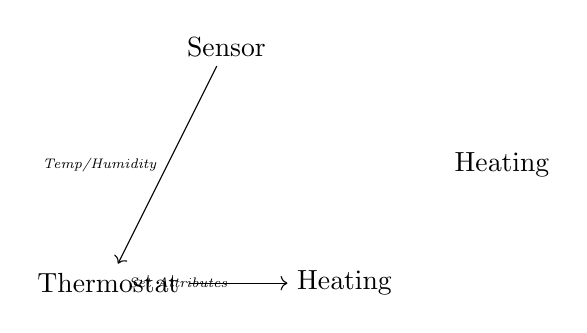
\begin{tikzpicture}
      \node[draw=white,align=left] (S) at (1.5,3) {Sensor};
      \node[draw=white,align=left] (T) at (0,0) {Thermostat};
      \node[draw=white,align=left] (H) at (3,0) {Heating};
      \node[draw=white,align=left] (E) at (5,1.5) {Heating};
      
      \path [->] (S) edge node[left] {\tiny \textit{Temp/Humidity}} (T);
      \path [->] (T) edge node[left] {\tiny \textit{Set Attributes}} (H);
      % \path [->] (H) edge node[left] {} (S);
   \end{tikzpicture}
   
   \caption{Heating System - exercise 2 Schema}
   \label{fig:zigbee_heatingsystem}
\end{figure}
\chapter{Networking}
The two key aspects of a network are:
\begin{enumerate}
   \item \textbf{Bandwidth} $\longrightarrow$ amount of data per second that can be moved through a specific connection
   \item \textbf{Latency} $\longrightarrow$ is the amount of time required for trasmitting data, measured from the moment it is sent from the source to the one it is available to the source.
\end{enumerate}
Latency ---in a datacenter--- to transmit data on the cable using \textit{``pure ethernet''} is of the order of $0.5\times10^{-6}s (\mu s)$.\\
If the TCP/IP stack is used (standard application case), latency is about $70-90\mu s$.

Furthermore, current drives have reached speeds such that latency may act as bottleneck between them and the CPU.

Cable aggregation (e.g. aggregating 4 cables 10Gbit/s, providing 40Gbit/s total)can be performed only at a low ---physical--- level. Otherwise the TCP/IP stream will be associated to a single cable of the ones aggregated, resulting in less bandwidth.

\section{SDN - Software Defined Networking}
SDN is a new approach to networking that uses software-based controllers or application programming interfaces (APIs) to communicate with the underlying hardware infrastructure and direct traffic on the network.

In general a Software Defined Approach aims to abstract all the infrastructure components (compute, storage and network), and pools them into aggregated capacity.

When such approach is applied to a whole datacenter, it is called \textbf{Software Defined Datacenter}, and it is a way to abstract all the infrastructure components in order to provide IT as a service.

\subsection{Hyperconverged Infrastructure (HCI)}
HCI is a software-defined IT infrastructure that virtualizes all of the elements of conventional hardware-defined systems. HCI includes, at a minimum, virtualized computing (a hypervisor), a virtualized SAN (software-defined storage) and virtualized networking (software-defined networking).

\section{Layers}
Programmers usually do not care about anything under layer 3/4 traffic.
However, in datacenters it is fundamental to understand how layer 2 works.
\note{Also because in datacenters there are no routers doing the work for you; you are building the fabric in the first place.}

Layer 2 is fundamental for 2 reasons:
\begin{enumerate}
   \item East-west is Ethernet in the datacenter
   \item All the dozens of protocols used in swithces are really used, so they are important.
   \item MTU - Maximum Transmission Unit
\end{enumerate}

\subsection{Protocols inside switches}
\begin{itemize}
   \item LLDP Link Layer Discovery Protocol - Allows to reconstruct at least partially the functioning of the network.4
   \item DCBX Data Center Bridging Exchange - A meta-protocol so that two devices can agree on the configuration of a bunch of protocols, tipically related to storage/data 
   \note{e.g. ``I need 50\% percent of the bandwidth otherwise a can't work''.\\
   It represents part of some kind of QoS for Ethernet}.
   \item PFC Priority Flow Control
   \item ETS Enhanced Transmission Selection
   \item RSTP Rapid Spanning Tree Protocol - Uses BPDU packets to explore the graph of the network and compute the spanning tree of the network and detect the ---malicious--- cycles if any.
\end{itemize}

This just to recall that \ul{the switch is not a stupid thing}! It is complex, fascinating, and deserves love; it's crucial to understand its functioning, also because its protocols occupy bandwidth.

\section{Ethernet Topology}
Typically nowdays the network is a \textbf{graph}, where internal nodes are switches or routers, and the leaves are servers.

The phyisical medium is no more shared, but conceptually the data link layer behaves as if it was.

On a switch, the only way to emulate a \textbf{shared bus}, is to \textit{``\textbf{copy-paste}''} a frame onto multiple ports, losing the ``identity'' of frames; there is not routing table at layer 2. Packets in higher layers (IP?) have an ID, but frames don't, making it impossible to recognize whether a frame is a copy of another one or not.
This approach makes \textbf{loops} a problem, because they disrupt performance by generating a packet storm.\\
The solution would be to ensure that the topology resembles a \textbf{tree}, instead of a graph.
\ul{But}, at the same time, \ul{a \textbf{fully connected graph}} allows to have \ul{multiple routes for the same destination}, possibly \ul{enhancing performance}, reducing ``hops'' before reaching the destination.

\subsection{\texttt{RSTP}}
\begin{center}
   \textit{So\dots how can we leave the graph to be connected, but making it a tree from a logical point of view?}

   The answer is the \texttt{RSTP} protocol.
\end{center}

RSTP sends \textit{probes} to understand whether there are loops and where are PCs located.
In case of link failure, RSTP is able to adjust the logical tree, blocking the link that caused the loop.

RSTP can be used in campus networks or other networks exhibiting primarily North-South traffic, but it is not suitable for datacenters, where the traffic is mainly East-West:
the protocol is too slow (order of \textit{seconds})to handle the high number of links and the high number of switches typical of a datacenter.

\subsection{Three-tier architecture}
\begin{paracol}{2}
   
   Simple architecture consisting of\ns
   \begin{enumerate}
      \item Core switches
      \item Aggregation switches
      \item Access switches
   \end{enumerate}\ns
   The switches are connected in a tree-like topology, with the core switches at the top, the aggregation switches in the middle, and the access switches at the bottom.\\
   STP is used to prevent loops in the network.

   Also provides active-passive redundancy which leads to inefficient east west traffic, because the traffic is forced to go through the core switches (?), and devices connected to the same port may contend for bandwidth.\\
   Moreover communication server-to-server might requires crossing between layer, causing latency and the abovementioned traffic bottleneck.
   
   \switchcolumn
   
   \colfill
   \begin{figure}[htbp]
      \centering
      \includegraphics{images/3tier_switches.png}
      \caption{Three-tier architecture schema}
      \label{fig:3tier_switches}
   \end{figure}
   \colfill
   
\end{paracol}
This architecture is not used anymore, because it is not scalable, and it is not able to handle the high number of links and switches typical of a datacenter; more specifically, it does not fit virtualization most crucial need to be able to freely move VMs between servers.

\subsection{Spine Leaf architecture}
\begin{figure}[htbp]
   \centering
   \includegraphics{images/spineleaf.png}
   \caption{Spine-leaf architecture schema (from \href{https://www.arubanetworks.com/faq/what-is-spine-leaf-architecture/}{Arubanetworks.com})}
   \label{fig:}
\end{figure}
A \textbf{spine-leaf} architecture is data center network topology that consists of two switching layers:
\begin{enumerate}
   \item \textbf{Spine layer}\\
   Swtiches responsible for routing traffic, working as the backbone of the network.   
   \item \textbf{Leaf layer}\\
   Switches connected to endpoints, such as servers, storage devices, firewalls, load balancers, edge routers, etc.
\end{enumerate}
Since \ul{every leaf switch is connected to every spine switch}, the spine-leaf architecture is a \textbf{fully connected} network,
ensuring that any source is always the same number of hops (actually only one \smiley) away from any destination, so latency is lower and predictable (fixed).

Capacity also improves because STP is no longer required. While STP enables redundant paths between two switches, only one can be active at any time. As a result, paths often become oversubscribed. 
Conversely, spine-leaf architectures rely on protocols such as \textit{Equal-Cost Multipath} (\texttt{ECMP}) routing to load balance traffic across all available paths while still preventing network loops.

Spine-leaf allows \textit{scale-out} opposed to \textit{scale-up}, by adding additional spine switches, ultimately increasing capacity in case the bandwidth is not enough; doing so reduces also the subscription

\subsubsection{LACP}
Loops are prevented using \texttt{LACP} (\textit{Link Aggregation Control Protocol}), which is a protocol that allows to aggregate multiple links into a single logical link, providing higher bandwidth and active-active redundancy (in case a link fails);
it also ensures no loops because each link is a single channel, and these are named \textit{port channels}.

LACP also provides a method to control the bundling of several physical ports together to form a single logical channel.

Note that even though the bandwidth is aggregated (i.e. $2\times 25Gbps$), the single stream is still limited to the bandwidth of a single link (i.e. $25Gbps$), because the traffic goes only from one way to the other each time.

\subsubsection{Advantages of Spine-Leaf}

\begin{itemize}
   \item Modular (because you can mix and match devices) with fixed size switches.
   \item Latency predictable: every host is distance one or two hops to each other host.
   \item Bandwidth control (it's possible to chose the proportion of NS and EW traffic) and overbooking (overbooking explained after).
   \item Active-active redundancy (because both links of the port channels are enabled, so is the LACP to decide)
   \item Loop aware topology (a tree topology with no links disabled for redundancy reasons).
   \item Interconnect using standard cables (decide how many links use to interconnect spines with leaves and how many others link to racks).
   
\end{itemize}
With this architecture it’s possible to turn off one switch, upgrade it and reboot it without compromising the network. Half of the bandwidth is lost in the process, but the twin switch keeps the connection alive.

A typical configuration of the ports and bandwidth of the leaves is:
\begin{itemize}
   \item 1/3 going upwards and 2/3 going downwards
   \item 48 ports 10 Gbps each (downward - from leaves to racks)
   \begin{itemize}
      \item plus 6 ports 40 Gbps each (upward - from leaves to spines)
   \end{itemize}
   \item or (typical switch) 48 ports 25 each (downward)
   \begin{itemize}
      \item plus 6 ports 100 each (upward)
   \end{itemize}
\end{itemize}

Just a small remark: with spine and leaf we introduce \textbf{more hops}, so more latency, than the chassis approach. The solution for this problem is using as
a base of the spine a huge switch (256 ports) which actually acts as a
chassis, in order to reduce the number of hops and latency.


\subsection{Full fat tree}
In a ---full?--- \textbf{fat tree}, branches nearer the top of the hierarchy are "fatter" (thicker) than branches further down the hierarchy. In a telecommunications network, the branches are data links; the varied thickness (bandwidth) of the data links allows for more efficient and technology-specific use.

Full-fat tree is rarely needed.

\section{Virtualization}

With VLAN frames are extended by 4 bytes. Every switch nowdays automatically sets the \texttt{VLAN\_ID} to \texttt{1}; if the field is not existent, it is appended, making an \textbf{tagged} an \textit{untagged} frame.

Switches ensure that data cannot spill/leak from a VLAN to another.
VLAN became largely of use when 10Gbit connection came out, because only 1Gbit was a too constrained bandwidth to be splitted into multiple VLANs. 

VLAN are used to partition the traffic at data link layer without having to redo the fabric. They are particularly useful in cloud environments.

\section{Network Administrator POV}
The switch is split in two planes:
\begin{itemize}
   \item \textbf{Control Plane}\\
   This plane is necessary to configure the data plane to make it behave according to our needs.
   Here there is an \textit{OS}, which used to be proprietary with a functioning fitting a specific network configuration, but nowdays they are usually more configurable and may even be \textit{open} OS.
   \note{\textit{Dell}'s switches now have an \textit{open} OS on board.}
   
   \item \textbf{Data Plane}\\
   Here lies the chip responsible to perform all the data link operations required, runs protocols, handles VLANs, etc.

   \textbf{OpenFlow} allows us to manage the flow table inside of a switch.
\end{itemize}

The two planes are linked by a low-bandwidth PCIe.


It is possible to use a very fast and simple ---reduced number of keystroke down to the strict necessary ones (e.g. \texttt{en} instead of \texttt{enable})--- CLI to program a switch. It is also possible to create a script file to be automatically executed by the switch at boot time.
\note{Prof. Cisternino performed a demo of this in class.}

Interestingly, the behaviour of the \texttt{netsh} command in Windows is very similar to the one of a switch.

\section{SDN}
\textbf{Software Defined Networking} is a new approach to networking that uses software-based controllers or application programming interfaces (APIs) to communicate with the underlying hardware infrastructure and direct traffic on the network.

The problem was that the network infrastructure was ``ossified'' and not programmable. SDN allows to program the network, and to make it more flexible and adaptable to the needs of the applications, without having to disrupt the existing infrastructure.

The key idea proposed in the OpenFlow article, which eventually became a standard, is to separate the control plane from the data plane, and to have a controller that can program through an API the data plane, where the \textbf{Flow Table} resides.

An interesting use of OpenFlow was implemented by a University and called Sandwich firewall, which consisted in routing the first part of the stream through a firewall and if the stream was not malicious, it was routed directly to the destination, otherwise it was dropped.

\subsection*{Latency-sensitive}
Some workloads are called \textit{latency-sensitive}, making the latency introduced by TCP-IP stack a problem.\\
Inside a datacenter nowadays the typical latency is sub microsecond.

Regarding this issue, technologies mentioned earlier come in handy; 
\textit{InfiniBand} is a fabric technology that allows to have a very low latency, and is used in HPC\footnote{High performance computing} environments, and \textit{OmniPath} is a technology that is similar to InfiniBand, but is more scalable and is its natural successor.
Also \textit{RDMA} and \textit{RoCE} are technologies that allow to access memory of a remote machine without involving the CPU or the OS of the remote machine, bypassing the TCP/IP stack.

\textit{Fibre Channel} switches are used in storage area networks, and are used to connect storage to servers CPUs. They are used in datacenters, but not for networking.
\chapter{Blockchain}
The basic concepts concerning Blockchains are
\begin{itemize}
   \item \textit{Ledger}
   \item \textit{Consensus} in a distributed environment
   \item Tamper freeness
   \item Proof of ownership
   \item Permissioned and permissionless blockchains
\end{itemize}

Each \textbf{block} is made up of \textit{Data}, \textit{Hash} and the \textit{Hash of the previous block}; pointers to the previous block are used to ensure the \textbf{order} of the blocks, resulting in a \textbf{chain} of blocks.

\textbf{Tamper freeness} refers to changing one hash causes changing the hash of the following blocks, implying not only to recompute some hashes, but also to find a value that combined with the new hash solves the \textit{Proof of Work}.

\begin{figure}[htbp]
   \centering
   \includegraphics{images/hashpointers.png}
   \caption{Hash pointers and hash of the block prevent attackers from tampering with the blockchain}
   \label{fig:hashpointers}
\end{figure}

A \textbf{ledger}\footnote{\textit{``Libro mastro''} in italiano} acts like a notary, and is replicated on each node of a P2P network, it is immutable and benefits of the tamper freeness property.\\
The ledger is like a bullettin storing operations and their order. It must be an \textbf{append-only} list of events, and also \textbf{tamper-proof}.

\begin{center}
   \ul{If a ledger is organized as a list of blocks, we call it a \textbf{blockchain}}.
\end{center}
\nl

\section{Consesus and challenges}
\textbf{Consensus} is the mechanism which defines who decides which operation will be added to the blockchain, and which operation among those to be confirmed will be added.
Consesus is implemented by \textit{voting}, but there a few things to handle to avoid double spending and fake votes.
\textit{Sybil} attacks are a common issue in voting systems, where a single node can fake multiple identities to gain more voting power.

The two main challenges for the ledger are keeping consistency in case of network jitter and possible delays, and avoid nodes to fake results.
An idea is to establish \textit{consensus} using a \textbf{Proof of Work}, which requires the voting system to be hardly fakeable, i.e. resolving a difficult computational problem.
Enforcing a \textit{PoW} is a way to avoid the Sybil attacks issue, as it implies to have a lot of computational power to fake a vote.\\
The Proof of Work is often compared to a lottery, where tickets for the lottery are very expensive (computational power), and the winner is the one who solves the problem first, and gets the right to decide which block to add to the blockchain.

In case multiple winners are picked at the same time, a \textbf{fork} is created, and the network must decide which fork to follow. The longest fork is usually the one to be followed, as it is the one with the most computational power behind it.

\section{Restricted access}
It is possible to build a permissioned blockchain, where only a restricted set of nodes can vote and add blocks to the blockchain. This is useful in case of a consortium of companies, where the blockchain is used to store transactions between them.

The blockchain may be exploited to demonstrate the validity of the supply chain of a product, or to store the history of a product, from the raw materials to the final product, allowing also to determine which point in the supply chain a product has been compromised.
\chapter{Reflection}
\section*{9 - Ottobre}
\section{Introduction and Definitions}

\textbf{Reflection} is the ability of a program to manipulate as data something representing the state of the program during its own execution.
Another dimension of reflection is if a program is
allowed to \textbf{read only}, or also to \textbf{change} itself.
\begin{itemize}
    \item \textbf{Introspection} is the ability of a program to observe and
    therefore reason about its own state
    \item \textbf{Intercession} is the ability for a program to modify its
    own execution state or alter its own interpretation or
    meaning
    \item \textbf{Reification} is the mechanism of encoding execution state into data, which is needed by both \textit{introspection} and \textit{intercession}
\end{itemize}.

\textbf{Structural} reflection  is concerned with the ability of the \textbf{language} to provide a complete \textit{reification} of both the \textit{program} executed and its \textit{abstract data types}.\\
\textbf{Behavioral} reflection is concerned instead with the reification of its\footnote{referred to a \textbf{language}} \textit{semantics} \& \textit{implementation} (processor) and the data and implementation of the \textit{run-time system}.

\section{Uses and drawbacks}
\subsection{Uses}
\begin{itemize}
    \item \textit{Class Browsers} need to be able to enumerate the number of classes
    \item \textit{Visual Development Environments} can exploit type info available in reflection to aid the developer in writing correct code
    \item \textit{Debuggers} need to be able to examine private members on classes
    \item \textit{Test Tools} exploit reflection to ensure a high level of code coverage in a test suite
    \item \textit{Extensibility Features} an app may make use of external, user-defined classes by creating instances of extensibility objects.
\end{itemize}

\subsection{Drawbacks}
\begin{itemize}
    \item \textbf{Performance Overhead}
    \item \textbf{Security Restrictions}
    \item \textbf{Exposure of internals}
\end{itemize}

\section{Reflection in Java}
Java supports \textbf{introspection} and \textbf{reflexive invocation},
but not \textit{code modification}.

\subsection{Introspection}

The JVM mantains for every type an associated object of type \lstinline{java.lang.Class} which "\textit{reflects}" the type it represents,
acting as entry point for reflection,
since it provides all info needed:
\begin{itemize}
    \item Class name and modifiers
    \item Extended superclasses and implemented inferfaces
    \item Methods, fields, constructors, etc.
\end{itemize}

To retrieve such \lstinline{java.lang.Class} object it is sufficient to do \lstinline{Object.getClass()}.
\lstinline{Class} objects are constructed automatically by the JVM as classes are loaded.

Using \lstinline{java.util.reflect.*} it is possible also to retrieve class \textbf{Members} i.e. \textit{fields, constructors} and \textit{methods}.
The extensive \lstinline{java.util.reflect.*} API provides many \textit{methods} to achieve this which will not be reported here.\\
There is a class for each Member
\begin{itemize}
    \item \lstinline{java.util.reflect.Field}: access type info and set/get values.
    \item \lstinline{java.util.reflect.Method}: type info for parameters and return type;
    invoking method on a given object.
    \item \lstinline{java.util.reflect.Constructor}: note that constructors have no return values and invocation creates a new instance of the given class.
\end{itemize}

\subsection{Program Manipulation}
By now we have talked only about \textbf{introspection} in java,
but reflection can be used also to create objects of a type not known at compile time,
or to access members (access fields or invoke methods) unknown at compile time.


\chapter{Virtualization}

Virtualization consists in virtualizing hardware resources, such as CPU, memory, storage, and network interfaces. This allows to run multiple operating systems on the same physical machine, which is called \textit{host}.

It is not equal to \textit{emulation} which consists in simulating hardware, giving the illusion that you are in another system, and is much slower than virtualization, since each instruction in the emulated system gets translated into up to ---possibly--- thousands  of instructions in the host.

\framedt{CPU Rings and isolation}{
   \ul{Virtualization is a strong way of isolating things.}\\
   To isolate VMs the hypervisor exploits CPU rings, which are used to separate the different levels of privilege. The higher the ring, the higher the privilege level.
   In intel CPUs there are 16 rings.
}

There are two kinds of virtualization systems:
\begin{enumerate}
   \item VirtualPC (Microsoft), VirtualBox (Oracle), VMware Workstation (VMware), Parallels (Apple) : these are \textit{desktop virtualization systems}, which are used to run multiple operating systems on the same physical machine.\\
   These solutions aim to provide ``interactive'' computers, with a GUI, peripheral support, etc. 
   \item VMware ESXi, Microsoft Hyper-V, KVM, Xen : these are \textit{server virtualization systems} (\textbf{HyperVisors}), which are used to run multiple servers, typically GUI-less, on the same physical machine.\\
   Hypervisors introduce a \textbf{crucial} piece of software called \textbf{Virtual Switch}, which is responsible for managing the network of the virtual machines.
   The virtual switch's uplink is the host's physical network interface.
\end{enumerate}
Similarly to snapshots in storage systems, there are \textbf{checkpoints}, which are used to save the state of a virtual machine at a certain point in time. This is useful to revert to a previous state in case of problems.

\section{Network}
HyperVisors introduce a \textbf{crucial} piece of software called \textbf{Virtual Switch}, which is responsible for managing the network of the virtual machines.\\
VMware is the leader in virtualization, but lately they have been changing pricings and licensing, which has made some customers unhappy.\\
\note{Broadcom is a chip manufacturer, and we might end up with virtualization software already inside the chip. }

VMware virtual switch is called \textbf{vSwitch}. It is a software-based switch that is responsible for managing the network of the virtual machines.\\
Every network interface of a virtual machine has its own MAC address, and may be connected to a vSwitch.
\note{An hypervisor may handle multiple vSwitches.}
From a network point of view, a virtual machine is just like a physical machine, assuming that the network card is in \textbf{promiscuous} mode, it can see all the traffic that is going through the vSwitch.

\section{Live Migration}
Hypervisors provide also the migration of virtual machines from one host to another, which is called \textbf{vMotion} in VMware. This is useful for load balancing, maintenance, etc. In Windows Hyper-V, this primitive is called \textbf{Live Migration}.\\
The migration is performed \textit{without any service interruption}, only some degradation in performance and network latency.
This also allows to move virtual machines from one host to another in case of hardware failure or phyisical maintenance.
Besides, by redunding VMs we may also live switch from an older to a newer version of the software, without users noticing.

Live migration can performed like a context switch, by saving the state of the virtual machine and restoring it on the other host. This is possible because the virtual machine is not aware of the underlying hardware, and the hypervisor is responsible for managing the hardware resources.\\
Assuming that the disk is shared, the migration is performed like so:
\begin{enumerate}
   \item The memory (and the registries) of the virtual machine is copied to the other host
   \item If the copied memory is sufficient, the new VM starts to run on the other host
   \item When data from the older memory host is requested, the virtual machine is paused, and the memory is copied again to the other host
   \item Once the VM has been totally transferred, memory and other components belonging to the old VM are freed
\end{enumerate}

vSwitches are also migrated, so that the network configuration is preserved. The old vSwitch may communicate with the new one, and if needed forward packets, until ARP tables are updated.

\subsection{Replication}
Replication is the process of copying data from one host to another, in order to have a backup in case of failure.\\
Happens the same way as live migration, but the virtual machine is not running on the other host.
\chapter{Bitcoin Mining}

Recall that the \textbf{distributed consesus} is a procedure to reach a common agreement in a distributed or decentralized multi-agent system;
it must ensure correct results even in presence of faulty nodes, network partitioning and byzantine faults\footnote{Nodes behaving maliciously}.
\note{Even though it is difficult to classify the method used by Bitcoin to achieve decentralization from a theoretical point of view, it works in practice.

\textit{``...is not purely technical, but it's a combination of technical methods and clever incentive engineering.''}
}

\section{Competing}
Every node holds a \texttt{MemPool} containing all Bitcoin transactions awaiting confirmation.
\ul{\textit{Conflicts} may happen there, not in the ledger}.
In case a node receives a double-spending transaction, it will keep the first one and discard the second one.\\
Nodes try to get transactions into the ledger, and \textbf{compete} to do so.
Nakamoto consesus is implemented like a ``lottery'' where the winner gets to add a block ---of valid transactions--- to the blockchain, and to send its neighbours the updated ledger. The process of competing to add transactions to the blockchain is called \textbf{mining}.

\subsection{Mining}
Mining process starts with filling a candidate block with transactions taken
from the memory pool (\texttt{MemPool}), and then building a block header (1000 times smaller than the block);
finally the node performs the Proof of Work.\\
So, while a single transaction may be built by anyone, blocks are built by miners, and include multiple transactions and the header.

\begin{paracol}{2}
   \ns
   The block header contains:
   \begin{itemize}
      \item Version
      \item Timestamp
      \item \texttt{mhash} The Merkle \ul{root} of the transactions in the block
      \note{Merkle tree is not explicitly represented in the block, it is built on demand.\\
      Any change to a transaction results in a change of \texttt{mhash}, consequently in a change of the hash of the whole block.}
      \item \texttt{hashprev} The hash of the previous block \textit{header}, and a hash pointer to the previous block
      \item PoW related fields:
      \begin{itemize}
         \item Target
         \item Nonce
      \end{itemize}
   \end{itemize}
   \switchcolumn

   \colfill
   \begin{figure}[htbp]
      \centering
      \includegraphics{images/bitcoin_blockheader.png}
      % \caption{}
      \label{fig:bitcoin_blockheader}
   \end{figure}
   \colfill

\end{paracol}

\framedt{Mining}{
   \begin{enumerate}
      \item Set \texttt{nonce = 0}
      \item Hash the \textit{block header} including the \texttt{nonce}
      \item \texttt{while (\texttt{hash} > \texttt{target})}
      \begin{enumerate}
         \item Increment \texttt{nonce}
         \item Hash the \textit{block header} including the \texttt{nonce}
      \end{enumerate}
   \end{enumerate}
   \textbf{Target} acts as \textit{threshold}, and represents the \ul{number of leading zeros the hash must have}.
   The nonce is 32 bit long, and even a slight increment on it changes the whole hash result.
}

\subsection{Consesus}
Node is selected to propose the next block in proportion to a resource that it is hard to
monopolize: in Bitcoin this resource is \textbf{computational power} and the selection is done on the basis of the Proof of Work.

The Consensus is \textbf{implicit}:
\begin{itemize}
   \item No collective distributed algorithm executed by the nodes
   \item No voting
   \item Selection of malicious nodes is also implicitily handled by the system
\end{itemize}

Even if the nodes may have occasionally an inconsistent view of the ledger (blockchain forks) consensus will eventually occur, the consistent ledger will eventually be the longest chain.
\note{This is true if the majority of the nodes are honest.}

\subsection{Proof of Work}
\begin{itemize}
   \item \texttt{d} - \textit{difficulty}: a positive number which is used to adjust the time to execute the proof
   \item \texttt{c} - \textit{challange}: a given string (the block header minus the nonce)
   \item \texttt{x} - \textit{nonce}: an unknown string
\end{itemize}

\begin{definition}[Proof of Work]
   A proof of work is a function $F_d(c,x) \rightarrow {\texttt{True,False}}$ satisfying:
   \begin{enumerate}
      \item \texttt{d} and \texttt{c} are \textit{fixed}
      \item $F_d(c,x)$ is \textit{fast to compute}, if \texttt{d}, \texttt{c}, and \texttt{x} are known
      \item instead, finding \texttt{x} so that $F_d(c,x) = \texttt{True}$ is computationally difficult, but feasible.
   \end{enumerate}
\end{definition}

The PoW is hard to solve because the computing output looks like a random 256-bit string where each bit is equally likely to be \texttt{0} or \texttt{1} independently of the other bits, so each output bit looks like coin flips (\texttt{0/1}).
There is no better way of finding the correct output than trying by \textbf{brute force}.\\
The probability $p$ that the block hash is below the target $T$ and average number of attempts $a$ to find a solution are:
\begin{align*}
   p=\frac{T+1}{2^{256}} & & a=\frac{1}{p}
\end{align*}

The system is resistant to Sybil attacks because the PoW is a scarce resource, and the cost of the attack is proportional to the whole computational power of the attacker, not to the number of identities they have.

\note{The Proof of Work is also used in other contexts to prevent spam, like in Hashcash, and to counter DoS attacks, by allowing users to access a service only after solving a PoW.

Email spam may be prevented through a PoW by adding a post stamp to each email message, and the receiver may decide to accept the message only if the PoW is valid.}

\subsection{Block propagation and incentives}
\subsubsection{Block propagation}
The mined block is broadcasted on the network, and each node receiving the block verifies that the PoW has been solved by hashing the block header and checking that the hash is less than the target.
It is easy to verify, without centralization points.\\
After the verification, the node adds the block to the blockchain and kicks out any conflicting transaction from \texttt{MemPool}.

\subsubsection{Incentives}
There are two mechanisms to incentivize the miners to be honest:
\begin{enumerate}
   \item \textbf{\ul{Block reward}}:
   a payment to the miner in exchange for the service of creating a block.\\
   Bitcoin mints new coins when a new block is mined, and is the only way to create new bitcoins.\\
   The reward is halved every 210K blocks ($\sim 4 \textit{ years}$), and the last block reward will be mined in 2140.
   \item \textbf{\ul{Transaction fees}}:
   for each transaction in the block the miner gets the difference between transaction inputs and outputs.\\
   It was voluntarily inserted to obtain a good ``quality of service'' from the miners.
\end{enumerate}

The first transaction in each block is called \ul{\textbf{coinbase transaction}, and is the one that mints new coins}: it includes the reward plus the transaction fees to the miner, and is not linked to any previous UTXO, but to a single ``dummy'' input.

\framedt{Mining Difficulty}{
   \begin{center}
      \textit{``To compensate for increasing hardware speed and varying interest in running nodes over time, the proof-of-work difficulty is determined by a moving average targeting an average number of blocks per hour. If they're generated too fast, the difficulty increases.''}\\
      -Satoshi Nakamoto
   \end{center}
   The difficulty is adjusted every 2016 blocks (about 2 weeks) to keep the block time around \textbf{10 minutes}.
   The difficulty is adjusted by changing the target, which is inversely proportional to the difficulty.
}

\framedt{Why 10 Minutes?}{
   \begin{center}
      \textit{``If broadcasts turn out to be slower in practice than expected, the target time between blocks may have to be increased to avoid wasting resources. 
      We want blocks to usually propagate in much less time than it takes to generate them, otherwise nodes would spend too much time working on obsolete blocks.''}\\
      -Satoshi Nakamoto
   \end{center}

   The 10 minutes target time is a trade-off between the time to propagate a block and the time to generate a new one.\\
   The goal was to allow time to propagate across the whole network before the next block gets mined, to avoid wasting resources.
}

Note that 10 minutes mining time means that no instantaneous transactions are possible, but the system is designed to be secure, not fast.
\note{e.g. you can't pay for an ice cream using bitcoin.}

\begin{figure}[htbp]
   \centering
   \includegraphics{images/bitcoin_targetcycle.png}
   \caption{Bitcoin target cycle}
   \label{fig:bitcoin_targetcycle}
   \note{A node can't avoid decreasing the target, since the other nodes would not validate its Proof of Work.}
\end{figure}

\note{Blocks are preferred over single transactions, because verification is faster and mining single transactions would overall require more mining work.}

\subsection{Tamper-freeness}
The blockchain is tamper-free because:
\begin{itemize}
   \item The PoW is hard to solve
   \item The PoW is easy to verify
   \item The PoW is a scarce resource
\end{itemize}

\newpage
It would take an \ul{unfeasible amount of power for an attacker to change a transaction in a block}, since it would imply that: 
\begin{enumerate}
   \item The root of the Merkle tree changes and so the block header
   \item The nonce of the block is no more valid
   \item Re-execute PoW to re-compute the right nonce for the new block
   \item In the next block the hash pointer to the previous block changes as well
   \item Nonce of the next block is no more valid
   \item Need to re-execute also on next block...
   \item ...and so on
\end{enumerate}

\section{Temporary Forks}

\begin{paracol}{2}
   
   \colfill
   \ul{Temporary forks may happen when two miners find a valid block at the same time}, and broadcast it to the network.
   The state of the blockchain is seen by the nework consists of two branches both
   originating from the same parent block.
   In this case both branches are legitimate, and is different from the double spending case, but still, \textit{which bitcoin are really spent?}
   \colfill

   \switchcolumn

   \colfill
   \begin{figure}[htbp]
      \centering
      \includegraphics{images/bitcoin_forks.png}
      \caption{Bitcoin temporary forks}
      \label{fig:bitcoin_forks}
   \end{figure}
   \colfill
\end{paracol}
   

Each miner node either receives block A or block C first, which are both valid, but different,
and then starts mining on the branch of the fork with the block it received first;
note that the two forks may grow indipendently, and the network may have multiple branches.
If a \ul{miner receives a block that makes the other fork longer, it \textit{abandons} the
shorter fork};
the transactions of the ``abandoned'' fork that were not approved in the winning fork are returned to the pool of ``not-yet-approved'' transactions.
\begin{definition}[6 Confirmation Rule]
   \label{def:6confirmation}
   Bitcoin approves a transaction finally only once there are at least \textbf{five} following blocks in the chain 
\end{definition}

\framedt{May the two chains extended perfectly in parallel, to equal height?}{
   It may be possible, but extremely unlikely in practice.
   The probability that this happens recursively, for a long period is very low,
   besides mining and the block propagation delay introduce randomness in the protocol that typically prevents this.

   Recall that each miner switches to mine on the longest branch it becomes aware of.
}

\begin{definition}[Nakamoto Consesus]
   Forks are \textit{eventually} resolved and all nodes eventually agree on which is the longest
   blockchain. The system therefore guarantees \textbf{eventual consistency}.
\end{definition}

\section{Mining technologies}
The main Bitcoin actors are:
\begin{enumerate}
   \item Reference client (Bitcoin Core)
   \item Full block chain mode
   \item Solo miner
   \item Lightweight (SPV) wallet
\end{enumerate}

Basically, the mining process is SHA computation which can be summarized as follows:
\begin{lstlisting}
   while (1)
      HDR[kNoncePos]++;
      if (SHA256(SHA256(HDR)) < (65535 << 208)/ DIFFICULTY)
         return;
\end{lstlisting}
To compute such hash, CPUs were initially used, then GPUs,GPU pools, FPGAs ---Verilog programmable hardware--- and now ASICs are used.
It is unclear what will ASICs successor be.
ASICs stands for Application Specific Integrated Circuits, and are hardware devices specifically designed to perform a task, e.g. mining.
For this task, they are faster and more efficient than CPUs and GPUs.

\subsection{Centralized Mining pools}
\label{sec:mining_pools}
\ul{Mining is a very risky task}, since it is very likely to spend a lot for mining hardware and eletricity without
obtaining a reward for a long time.
\textbf{Mining pools} are a way to share the risk and the reward among the participants. 

The \textbf{Pool Manager} sends blocks to miners and distributes the reward among the participants, based on the work they have performed; it must be trusted by anyone.
\labelitemize{\textit{Challenges}}{
\begin{itemize}
   \item How does a pool manager know how much work each member of the pool is actually performing?
   \note{Also miners that have not been able to solve the PoW have to be rewarded for their work.}
   \item How can the pool manager divide the revenue proportional to the amount of work each miner is doing?
   \note{Partecipants to the pool may cheat, i.e. claim that they've done more than they actually did.\\
   It is in general hard to prove how much work a node has performed. Generally some ``near-valid blocks'' are sent to the pool manager, to indicate that the miner is actually working.}
\end{itemize}   
}

\textit{Pay-per-share} (PPS) is a common reward system used by mining pools, where the pool manager pays a fixed amount for each share submitted by the miner.
Miner's are payed from pool's existing balance, and there is no special reward for the miner who actually mines the block.

\textit{Pay-proportional} is instead a reward system where the pool manager enacts a reward proportional to the amount of work done by the miner, making miners more incentivized to present valid blocks.
This is less riskful for the pool manager, since payment is enacted only when a block is mined.
\note{\ul{Understading the amount of work done by a miner is still a challenge}. \textit{Decentralized mining pools} are a solution to this problem.}

\newpage
\subsection{Decentralized Mining pools}
\begin{paracol}{2}
   
   The basic idea behind decentralized mining pools is to build a separate, private chain including \textit{``weak blocks''} mined with lower difficulty, store in the private chain called \textit{``sharechain''} transactions rewarding for mining weak blocks
   until a valid block is found;
   at that point reward is distributed through a side blockchain which is then merged to the main chain, hence obtaining a transparent and fair payout scheme with efficiency minimal performance overhead.

   This approach also solves the problem of having a centralization point, since the pool manager does not have to be distribute the rewards.

   \switchcolumn
   \colfill
   \begin{figure}[htbp]
      \centering
      \includegraphics{images/bitcoin_decentralized_pool.png}
      \caption{Sharechain and main bitcoin chain}
      \label{fig:bitcoin_decentralized_pool}
   \end{figure}
   \colfill

\end{paracol}
\chapter{Embedded Programming}
The learning objectes of this chapter are embedded systems in general, and the Arduino case study.

\chapter{Replication}

\begin{definition}
   [Replication]
   Replication is the process of sharing information so as to ensure consistency between redundant resources, such as software or hardware components, to improve reliability, fault-tolerance, or accessibility.

\end{definition}


% // TODO up to leaders and followers

\section{Replication Fashions}
Each node may store a copy of the database, in this case it is called a \textbf{replica}, so, ensuring consistency among replicas is crucial.


\subsection{Leaders and followers}

\subsection{Synchronous vs Asynchronous Replication}
\begin{itemize}
   \item \textbf{Synchronous} - The leader waits for the followers to acknowledge the write before acknowledging the write itself.
   \begin{itemize}
      \item Ensures that followers have an up-to-date copy of the data.
      \item The disadvantage is that the system may become unavailable if a follower is slow to respond.
   \end{itemize}
   \item \textbf{Asynchronous} - The leader does not wait for the followers to acknowledge the write before acknowledging the write itself.
   \begin{itemize}
      \item Follower may fall behind the leader.
      \item The advantage is that the system continues processing even if a follower is slow to respond.
   \end{itemize}
   \item \textbf{Semi-synchronous} - The leader waits for a quorum of followers (at least one follower, typically always the same and placed in another location) to acknowledge the write before acknowledging the write itself.
   \begin{itemize}
      \item Ensures that at least one follower has an up-to-date copy of the data.
      \item Typically there is \ul{only one node fully synchronous}, while others are asynchronous, and it is \ul{placed far away from the leader}.
   \end{itemize}
\end{itemize}

\section{Failure}
\begin{itemize}
   \item Node failures - Nodes can fail due to faults or planned maintenance. The goal is to minimize impact and keep the system running.
   \item Follower failure: Catch up recovery - Followers keep a log of data Challenges //TODO
   % // TODO
   \item Leader failure: Failover - 
   \item Challenges in Failover -
\end{itemize}

\subsection{Implementing Replication Logs}
\begin{itemize}
   \item \textbf{Statement-based} replication - Replicate SQL write requests statements from the leader to the followers.
   \note{We cannot ensure a fully consistent system, due to issues with non-deterministic functions, autoincrementing columns, and side effects.\\
   This was used in VoltDB and MySQL before version 5.1.}
   \item \textbf{Write-ahead log (WAL)} shipping - Replicate the log of changes to the database from the leader to the followers.
   \note{Still some problems here, because we assume that the leader and the followers are using the same database engine, same architecture an so on, so that the log is the same.}
   \item \textbf{Logical log} replication - Replicate a logical representation of changes to the database from the leader to the followers.
   \note{This is advantageous and flexible, but it is dischouraged by the fact that some expertise and coding are required. Instead, with the first two approaches there is no need to modify the database in any way.}
   \item \textbf{Trigger-based} replication - Replicate changes to the database by using triggers.
\end{itemize}


\section{Eventual Consistency}
The eventual consistency model implies a temporary state where the followers lag behind the leader, but eventually they will catch up. 
Hence there is some ``replication-lag'' \dots
% //TODO

\subsection{Read-after-write consistency}
In asynchronous replication it is not trivial to ensure \textit{read-your-write} consistency, i.e. if a client writes a value to the leader, it should be able to read it.
In other words, a user may think their data is lost, because they cannot see it, but it is actually there, just not yet replicated to the follower.

\textit{Read-after-write} consistency guarantees that \ul{users see their own updates, but not necessarily the updates of others.}
It may be implemented by reading user-modified data from the leader.

\subsection{Monotonic Reads}
\textit{Monotonic reads} consistency guarantees that if a user has read the value of a key, it will not read an older value of the same key in the future.
It is stronger than eventual consistency, but weaker than strong consistency.

In asynchronous replication may see data moving backward in time when reading from different replicas with varying lag.\\
Monotonic reads can be achieved by ensuring that reads are always performed on the same replica.

\subsection{Consistent Prefix Reads w/different DBs}
\textit{Consistent prefix reads} consistency guarantees that if a sequence of writes happens in a certain order, then a read will see those writes in the same order.

Suppose that $A$ asks $B$ something, and $C$ is listening, but hears first the answers and later the question: weird, ain't it?\\
This may happen due to replication lag. We want to prevent casuality violations.


\section{Multi-Leader Replication}
With a single-leader configuration, the leader is a bottleneck, and if it fails, the system elects a new leader (perhaps there may be a small downtime).

With multi-leader replication, there are multiple leaders, and each leader can accept writes. This is useful for geographically distributed systems, where each region has its own leader.

\subsection{Collaborative Editing}
Real-time collaborative editing is a use case for multi-leader replication.\\
Changes are instantly appied to the user's local replica and then asynchronously replicated to the server and other users.

Application must obtain a lock on the document before editing, as with single leader replication with transactions (?).\\
The unit of change may be small, as a single keystroke.\nl

When two users edit the same part of the document, they get local updates, but when the system asynchronously synchronizes the replicas, a conflict occurs and needs resolution.\\
With single-leader replication, the second writer blocks or aborts if first write is incomplete, having the user to retry the input.\\
With multi-leader replication, the system must resolve the conflict, and the user must be notified of the resolution.

\subsection{Conflict Avoidance}
\labelitemize{Strategies}{
   \begin{itemize}
      \item Routing writes towards the same leader prevents conflicts.
      \item Routing user requests towards the same datacenter
      \item // TODO
   \end{itemize}
}

% // Prof SKIPPING a few slides starting from "consistent and converging to a state"


% // TODO
\subsection{Topologies}
\begin{itemize}
   \item \textbf{Circular} - each node receives writes and forwards writes
   \item \textbf{Star topology} - root node forwards writes to all other nodes 
   \item \textbf{All-to-all} - every leader sends writes to every other leader
\end{itemize}

Note that this is not hardware (neither virtual) network, but a logical network of replication, made up by how we manage the information flow.

In whatever topology it is important to \textbf{monitor staleness}, which is monitoring obsolete replicas, i.e. how far behind a follower is from the leader.
\chapter{Countermeasures}
\section*{20 - Ottobre}
\section{Robust Programming}
Ideally it indicates a programming style focused on minimizing vulnerabilities and the impact of any vulnerability still exploitable.

\textbf{Robust programming} can be summarized with a few guidelines:
\begin{enumerate}
   \item \textit{Validate} program inputs aka input is evil
   \item \textit{Prevent} buffer overflow aka check sizes
   \item A robust implementation minimizes any \textit{information leaked outside} 
   e.g. module, object, function ...
   \note{
      \begin{itemize}
         \item Logical pointers rather than physical ones
         \item Validate any information that is exchanged
      \end{itemize}
   }
   \item Check values transmitted to other functions (egress filtering)
   \item Check returned results
\end{enumerate}
Besides, it is important to focus also on \textbf{interaction controls},
robustness must be enforced on both malicious and erroneous behaviour.

\subsection{Input validation}
Usually input validation is achieved with a form of \textit{default \textbf{deny}} by defining a legal input structure and discarding every input which doesn't satisfy it.
\note{In case of string this may be done through RegEx, max length, ...}

It is important that the checks to validate the input should be specified when the program is designed rather than after an attack;
besides a check should be designed in an simple and readable way,
to easily ensure its correctness.
Some examples of input which usually must be validated are:
\begin{itemize}
   \item Environment variables
   \item File names (blanks, .., /)
   \item Email addresses
   \item URL
   \item HTML headers/body
   \item Data
\end{itemize} 

Memory allocation and strings length is a crucial aspect:
only library functions with an explicit string length specified should be used\footnote{e.g. \lstinline|strncpy()| instead of \lstinline|strcpy()|},
and in general,
it is appropriate to
allocate only the memory actually needed by a data structure according to its sizeto avoid leaving
space to store dangerous values or inputs.\nl

Speaking of functions,
attention must be paid to a rigorous \textbf{interfaces definition} and to avoid making assumptions on relationships between input and output values of function;
in other words, if a function $A$ takes as input the value $x$ returned by $B$,
it must not be \textit{asserted} that $x$ is for sure a \textbf{valid} value,
$B$ should check the correctness of the input regardless of knowing how it was generated.

\subsection{CWE - Vulnerabilities Ranking}
\href{https://cwe.mitre.org/top25/archive/2023/2023_top25_list.html#tableView}{This article} by \textit{\textbf{CWE}} (\textit{Common Weaknesses Enumeration}) lists the most dangerous and frequent software weaknesses of 2023,
based on data provided by \textit{NIST}.

The scoring formula to calculate a ranked order of weaknesses
considers the \textbf{frequency} a CWE is the root cause of a vulnerability
with the \textbf{severity} of its exploitation. Both frequency and severity are
\textit{normalized} relative to the minimum and maximum values seen.
\textbf{Frequency} is obtained by counting weaknesses occurences in the \textit{National Vulnerabilities Database} (NVD),
while \textbf{severity} is the average computed on the Vulnerabilities score in the \textit{CVSS}\footnote{\textit{Common Vulnerabilities Scoring System}} a given weakness is mapped to.\\
The \textbf{final weakness score} is computed by multiplying frequency and severity scores.

\subsubsection{Biases and limitations}
There are two biases which CWE doesn't take into account,
which somehow negatively affect how valid CWE's scores are:
\begin{enumerate}
   \item \textbf{Metric bias}
   \begin{enumerate}
      \item 
      Indirect prioritization of implementation faults over design flaws
      \item 
      Prefers frequency over severity due to distributions of real-world
   \end{enumerate}
   \item \textbf{Data bias}
   \item \begin{enumerate}
      \item Only uses NVD data based on publicly-reported CVE Records
      \item Many CVEs do not have sufficient details to assign a CWE
      mapping, omitting them from ranking
      \item There may be an over-representation of certain programming
      languages, frameworks, or weakness-detection techniques
   \end{enumerate}
\end{enumerate} 

There also a few aspects which this scoring system cannot represent and should be taken care of.
First of all,
weaknesses that are rarely discovered will not receive a high score,
regardless of the consequence of an exploitation.
Weaknesses that begin with a root cause of a mistake leading to
other mistakes, create a chain relationship.
As we have seen, chains of mistakes/vulnerabilities/attacks are a key point in security,
but CWE's scoring system treats any $\langle V_1, V_2 \rangle \wedge V_1 \rightarrow V_2$ as if $V_1$ and $V_2$ were independent i.e. $V_1 \not\rightarrow V_2$.


\section{Firewall}
A \textbf{firewall} is a module to filter all the messages exchanged by \textit{two} networks with a distinct security level;
\textit{all and only} the messages travelling on the wires
connecting the two networks cross the firewall and therefore get filtered.
A firewall works correctly under the assumption that a network has been split (\textit{segmented}) into two \textbf{subnets}, 
and that it \textit{correctly implements} a security policy, which should \textit{\textbf{not}} define the policy by itself.
Firewalls are usually \textbf{classified} on the known and manageable \textbf{protocols} and on their \textbf{implementation}.

\subsection{Segmenting}
Firewalling goes along with \textbf{segmenting} a network,
which results in multiple subnets with different security levels whose interaction is determined by firewalls inbetween them.
This architecture increases \textbf{robustness} by preventing an attacker from having \textbf{initial access} on an entire system and from freely performing \textbf{lateral movements};
besides this architecture perfectly integrates with \textbf{honeypot} deception mechanisms.

\subsection{Classification}
Firewall may operate on different levels of the TCP/IP stack and in different ways:
\begin{itemize}
   \item Packet filtering firewall
   \item Circuit-level gateway
   \item Application-level gateway (aka \textit{Proxy Firewall}):
   firewall which recognizes application level protocols and can make assumptions on it
   \item Stateful inspection firewall
   \textit{Stateful} means that the firewall inspects also the contents of a communication and the properties related to the status of a connection.
   \item Next-generation firewall (NGFW)
\end{itemize} 

At level 3 (IP Packet Inspection) the firewall can check only the header of IP packets,
while at level 4 (circuit level firewall) ...\nl

TODO\nl

\subsection{Pros \& Cons analysis}

\subsubsection{Packet-filtering firewall}
\begin{paracol}{2}
   \vspace{\fill}
   \labelitemize{
      \textit{Pros}
   }{
      \begin{itemize}
         \color{darkgreen}
         \item A Single device can filter traffic for an entire network
         \item Extremely fast and efficient in scanning traffic
         \item Inexpensive
      \item Minimal effect on other resources, network performance and end-user experience
      \end{itemize}
   }
   \vspace{\fill}
   \switchcolumn
   \vspace{\fill}
   \labelitemize{
      \textit{Cons}
   }{
      \begin{itemize}
         \color{darkred}
         \item Since traffic filtering is entirely based on IP addresses and ports,
         it lacks broader context that informs other types of firewalls
         \item Doesn't check the payload and can be easily spoofed
         \item Not an ideal option for every network
         \item Access control lists can be difficult o set up and manage
      \end{itemize}
   }
   \vspace{\fill}
\end{paracol}

\subsubsection{Circuit-level gateway}
\begin{paracol}{2}
   \vspace{\fill}
   \labelitemize{
      \textit{Pros}
   }{
      \begin{itemize}
         \color{darkgreen}
         \item Only processes requested transactions; all other traffic is rejected
         \item Easy to set up and manage
         \item Low cost and minimal impact on end-user experience
      \end{itemize}
   }

   \vspace{\fill}
   \switchcolumn
   \vspace{\fill}
   \labelitemize{
      \textit{Cons}
   }{
      \begin{itemize}
         \color{darkred}
         \item No protection against data leakage from devices within the firewall that should be used in conjunction with other security technology
         \item No application layer monitoring
         \item Requires ongoing updates to keep rules current
      \end{itemize}
   }
   \vspace{\fill}
\end{paracol}


\subsubsection{Stateful inspection}
\begin{paracol}{2}
   \vspace{\fill}
   \labelitemize{
      \textit{Pros}
   }{
      \begin{itemize}
         \color{darkgreen}
         \item Monitors the entire session for the state of the connection, while also checking
         IP addresses and payloads for more thorough security only layer 4 information
         \item Offers a high degree of control over what content is let in or out of the network
         \item Does not need to open numerous ports to allow traffic in or out
         \item Delivers substantive logging capabilities
         \item Some defence against DOS
      \end{itemize}
   }
   \vspace{\fill}
   \switchcolumn
   \vspace{\fill}
   \labelitemize{
      \textit{Cons}
   }{
      \begin{itemize}
         \color{darkred}
         \item Resource-intensive and interferes with the speed of network communications
         \item More expensive than other firewall options
         \item No authentication capabilities to validate traffic sources aren't spoofed
      \end{itemize}
   }
   \vspace{\fill}
\end{paracol}
Most popular firewall as it acts as a gateway between computers and other assets
within the firewall and resources beyond the enterprise

\subsubsection{Application-level}
\begin{paracol}{2}
   \vspace{\fill}
   \labelitemize{
      \textit{Pros}
   }{
      \begin{itemize}
         \color{darkgreen}
         \item Examines all communications between outside sources and devices behind the
         firewall, checking not just address, port and TCP header information, but the
         content itself before it lets any traffic pass through the proxy. Layer 7 analysis
         \item Provides fine-grained security controls that can, for example, allow access to a
         website but restrict which pages on that site the user can open
         \item Protects user anonymity
   \end{itemize}
   }

   \vspace{\fill}
   \switchcolumn
   \vspace{\fill}
   \labelitemize{
      \textit{Cons}
   }{
      \begin{itemize}
         \color{darkred}
         \item Can inhibit network performance
         \item Costlier than some other firewall options
         \item Requires a high degree of effort to derive the maximum benefit from the
         gateway
         \item Doesn't work with all network protocols
      \end{itemize}
   }
   \vspace{\fill}
\end{paracol}
NGFWs are an essential safeguard for organizations in heavily
regulated industries, such as healthcare or finance

\subsubsection{NGFW}
\begin{paracol}{2}
   \vspace{\fill}
   \labelitemize{
      \textit{Pros}
   }{
      \begin{itemize}
         \color{darkgreen}
         \item Combines DPI with malware filtering and other controls to provide an
         optimal level of filtering. Considers also sender addresses
         \item Tracks all traffic from Layer 2 to the application layer for more
         accurate insights than other methods
         \item Can be automatically updated to provide current context
   \end{itemize}
   }
   \vspace{\fill}
   \switchcolumn
   \vspace{\fill}
   \labelitemize{
      \textit{Cons}
   }{
      \begin{itemize}
         \color{darkred}
         \item In order to derive the biggest benefit, organizations need to integrate
         NGFWs with other security systems, which can be a complex process
         \item Costlier than other firewall types
      \end{itemize}
   }
   \vspace{\fill}
\end{paracol}
NGFWs are an essential safeguard for organizations in heavily
regulated industries, such as healthcare or finance

\subsection*{Proxies}
\textbf{Proxies} protect clients from attacks from an external server,
while \textbf{reverse proxies} protect internal servers from attacks by external agents, 
besides they can also act as a load balancer.

\subsection{Wrapping Up}
\textbf{Stateful inspection} is the most common technology:
it works at the network layer and provides
dynamic packet filtering.
While packet filtering examines information in a
packet header, stateful inspection tracks each connection traversing any
firewall interface and confirms they are valid.
It is a system backed up by a state table that
tracks all sessions and inspects all packets passing through: 
if packets have
the properties the state table predicts, they can pass, otherwise they don't.
Clearly the state table changes
dynamically according to traffic flow.

\begin{figure}[ht]
   \centering
   \includegraphics{images/firewall_comparison.png}
   \caption{Brief Firewall families comparison}
   \label{fig:firewall_comparison}
\end{figure}

\subsection{Takeaway guidelines}
These are the guidelines according to SNAS which indicate "suspicious" traffic \textbf{outgoing} from your network,
thus the network traffic which should be \textbf{egress-filtered}.
\begin{itemize}
   \item All traffic directed to IP addresses in your network(or that you manage)
   \item MS RPC (TCP/UDP 135), NetBIOS/IP (TCP/UDP 137-139), SMB/IP (TCP/445)
   \item Trivial File Transfer Protocol - TFTP (UDP/69)
   \item Syslog (UDP/514)
   \item Simple Network Management Protocol – SNMP (UDP 161-162)
   \item SMTP from all but your mail server
   \item Internet Relay Chat IRC (TCP 6660-6669)
   \item ICMP Echo/Reply
   \item ICMP Host Unreachable
\end{itemize}

\section{Segmentation}

A \textbf{segmented} network forces an attacker to adopt \textbf{pivoting},
which is attacking a host only to exploit it to route traffic to other nodes or subnets,
usually this is achieved with the aid of a \textbf{beacon} to remotely control the host.
Hence, in general, segmentation leads the attacker to implement \textit{more} attacks.

\begin{figure}[htbp]
   \centering
   \includegraphics{images/pivoting.png}
   \caption{Segmented network and the need for Pivoting}
   \label{fig:pivoting}
\end{figure}

The attacker needs to perform pivoting to intrude in the network, thus they need to attack at least one host in left subnet and one in the right subnet;
otherwise they'd need to attack the firewall, but generally this is more costful in terms of effort and resources.

It is also possible to combine \textbf{firewalls} and \textbf{honeypots}.
They can be placed either in the internal network amongst other nodes or between the router and the global/outside network.
\chapter{Security and Privacy}
\begin{figure}[htbp]
   \centering
   \includegraphics{images/security_threats.png}
   \caption{Security threats}
   \label{fig:security_threats}
\end{figure}
\textbf{Security} is a \textit{system-wide issue}:
Application software depends on operating system, web server, language run-time system, database, frameworks and tools, which may \textit{all} be targeted by attacks.

There are some system management procedures whose aim is to increase security, 
the most obvious ones are \textbf{authentication} and \textbf{authorization} (later discussed in Sections \ref{sec:authentication} and \ref{sec:authentication}).
\textit{System infrastructure management} aims to keep infrastructure software configured
and to promptly apply security updates patching vulnerabilities.
Regularly \textit{monitoring attacks} enhances the ability to detect them and trigger resistance strategies to minimize the impact.
To achieve resilience instead, \textit{backup policies} are defined to keep undamaged copies of program and data files to be restored after an attack.
\section{Attacks types}

\subsection{Injection Attacks}
Malicious users try to crash the system by sending invalid input values.
The defense is definining a robust input validation.

\labelitemize{
   \textit{Examples}
}{
   \begin{enumerate}
      \item Buffer overflow attacks
      \item SQL Poisoning
   \end{enumerate}
}

\subsection{Session hijacking}
A \textit{Session} is a time period during which user's auth with a web app is valid;
it allows the user to not having to re-authenticate for subsequent system interactions.
A session is closed when the user logs out or due to a “times out” caused by
no user inputs for some time. 

An attacker may acquires a valid session cookie through \textit{Cross-site scripting} (\textit{active} hijacking) or \textit{traffic monitoring} (\textit{passive} hijacking), and then impersonate a legitimate user.

Possible defenses include:
\begin{itemize}
   \item Encryption (\texttt{HTTPS})
   \item Multifactor authentication
   \item Short timeout sessions
\end{itemize}

\subsubsection{Cross-site Scripting}
\texttt{XSS} (i.e. \textit{cross-site scripting}) falls in the category of injection attacks,
since it consists in adding malicious code {---}to leak information{---} to a web page returned from a server to a user,
which inputs precious data handled by the malware.

\subsection{Denial-of-Service attacks}
\textbf{DoS} are intended to make system unavailable for normal use,
and were typically implemented by sending a high number of requests to overload servers,
resulting in the unavailability of services provided by such servers.

An historical \textbf{DoS} technique exploited the TCP 3-way handshake.
DoS developed in \textit{Distributed DoS} (\textbf{DDoS}),
i.e. sending requests from multiple IP addresses.

The most basic DoS techniques now have standard countermeasures to block them.
Widely used basic countermeasures include:
\begin{enumerate}
   \item IP tracking
   \item Temporary users lockout after failed authentication
\end{enumerate}

\subsection{Brute Force}
Attackers may try to guess missing authentication information by generating all possible combinations of characters,
possibly by knowing partial information on the string to be generated.


\section{Authentication}
\label{sec:authentication}
\labelitemize{
   \textit{Approaches}
}{
   \begin{enumerate}
      \item \textbf{Knowledge}-based authentication\\
      Personal secret knwon by the user.\\
      Passwords are often insecure, forgotten, reused,
       and besides the user can be fooled into inserting it in fake websites (\textit{phishing}).
      \item \textbf{Possession}-based authentication\\
      Possessing a physical device which provides tokens.
      \item \textbf{Attribute}-based authentication\\
      Biometric information of the user.
      \item \textbf{Multi-factor}:\\
      Combining the above. 
      This is becoming way more common and standardized.
   \end{enumerate}
}

Some services provide a \textbf{federated} authentication method e.g. \textit{"Login with Google"}, typically implemented using library \texttt{OAuth},
which rely on a trusted third party authenticator;
such method is widely used on mobile devices, where typing passwords is inconvenient,
but in general can fit in many scenarios,
with the downside of forcing the product provider to share some data with the (external) authenticator.

\section{Authorization}
\label{sec:authorization}
\textbf{Authorization} involves checking that an authenticated user can \textit{access resources},
while \textbf{authentication} is only about ensuring that the user is who they claim to be.

\textit{Access Control Lists} (\texttt{ACL}s) are widely used to implement access control policies,
they allow
classifying individuals into groups, dramatically reducing ACLs size,
and definining hierarchies of groups.\\
ACLs often realized by relying on ACL of underlying file or db
system.

\section{Encryption}

Encryption means making a document unreadable by applying an algorithmic transformation to it.
Modern encryption techniques are considered “practically uncrackable”
using currently available technology.

There are well-known symmetric and asymmetric encryption techniques.
\texttt{HTTPS} uses server-client interaction to generate a secret for symmetric encryption.\\
$\texttt{HTTPS} = \texttt{HTTP} + \st{\texttt{SSL}}\ \texttt{TLS}$ \textit{(Transport Layer Security)}\\
TLS is used to verify \textit{identity} of web server and to encrypt communications,
it does so by exploiting a digital certificate sent from server to client, issued by a trusted identity verification service (\texttt{CA}).

In general encryption should be adopted \textbf{whenever possible},
for both \textit{in transit} and \textit{at rest} data,
while for \textit{in use} data it is known that may cripple performance, 
and mechanisms of key management are used instead.

Ideally, if keys get lost, encrypted data become permanently inaccessible.
Keys should be changed periodically and multiple timestamped versions of keys should be mantained,
creating the need for a \textbf{Key Management System}
(\textit{KMS}) to make sure that keys are securely generated, stored, and accessed by authorized users.

\begin{figure}[htbp]
   \centering
   \includegraphics{images/encryption.png}
   \caption{Encryption is possible in all system levels}
   \label{fig:encryption}
\end{figure}

\section{Privacy}
\textbf{Privacy} is a social concept that relates to the collection,
dissemination, and appropriate use of personal information held
by a third party.

There may business reasons for paying attention to information privacy:
\begin{itemize}
   \item If your conformance to privacy regulations does not match data
   protection regulations, you may be subject to legal actions / cannot sell
   your product
   \item If your sell a business product, your business customers may require privacy safeguards (not to be at risk with their users)
   \item Leakage/misuse of client information can damage your reputation
\end{itemize}

The information that your software \textit{needs} to collect depends on the
\textit{functionality} of your product and on the business model you use;
we can provide some tips based on this assumption:
\begin{itemize}
   \item Do not collect personal information that you do not need
   \item Establish a privacy policy defining how personal/sensitive information about
   users is collected, stored, and managed
   \item Make clear if you use users’ data to target advertising or to provide services that are paid for by other companies
   \item If your product includes social network functionalities so that users can share
   information, you should ensure that users understand how to control the
   information they share
\end{itemize}

\section{Microservices}
In microservices there is much inter-service communication via remote calls and thus a large number of entry points, 
considerably broadening the \textbf{attack surface}.
Besides, each microservice requires carrying out an individual \textbf{security screening},
to assess changes in time, given the mutable structure of this architetural style.
\note{The most used approach is \textit{ZeroTrust} networks, which {--}sadly{--} have some impact on performance}

\subsection{Communication}
Service-to-service communication must take place on \textit{protected channels}, and typically exploits the use of \textbf{certificates}, \underline{one for each microservice.}
Even though it's effective,
revoking and rotating certificates on hundreds of microservices is a complex task, and thus should be automated.

\subsection{Logging}
A request to a microservices deployment may span multiple microservices, making correlating requests among microservices challenging.
To this extent logs and traces help a lot:\\
\textbf{Logs} can be aggregated to produce metrics that reflect system state (e.g.
average invalid access requests per hour) and that may trigger alerts on security or performance;
\textbf{Traces} instead help you tracking a request from the point where it enters the system to the point where it leaves the system.
\note{
   \begin{itemize}
      \item \textbf{logging}: 
      \textit{Prometheus} and \textit{Grafana} to monitor incoming requests
      \item \textbf{Tracing}:
      \textit{Jaeger} and \textit{Zipkin} for distributed tracing
   \end{itemize}
}

\subsection{Containers against statefulness}
Containers are \textit{\underline{immutable} servers}, they don’t change state after being spinned up;
This is a great property which simplifies deployment and allows horizontal-scalability,
but for each service we need to maintain a \textbf{dynamic list} of allowed clients and a dynamic set of access-control policies, which \textit{cannot} be stored inside the container.
A solution is to use a \texttt{push/pull} model to get updated policies from some policy admin endpoint.\\
Each service must also maintain its own \textbf{credentials}, which need to be rotated periodically,
but this can be handlend by keeping credentials in container filesystem, by injecting them at \textit{boot time}.

Since containers have no state, and requests span distributedly, \textbf{user context} has to be \textit{passed explicitly} from one microservice to another,
so there must be a way to ensure trust between microservices so that receiving microservice accepts user context passed from calling microservice.
\note{Typically implemented with \textit{JSON Web Tokens} (\texttt{JWT})}

\note{
   \paragraph*{Confused Deputy}
   What is the “confused deputy problem“ in microservices?
   \begin{enumerate}
      \item application does not enact access control in some microservices, allowing the attacker to get data it shouldn’t be able to get
      \item microservices trust the gateway based on its mere identity, leading to potential violation of authenticity
   \end{enumerate} 
}
\subsection{Architetural smells}
\begin{table}[htbp]
   \centering
   \begin{tabular}{|c|c|c|}
      \toprule
      \textbf{Property} & \textbf{Smell} & \textbf{Solution}\\
      \midrule
      Confidentiality & Insufficient Access Control & \texttt{OAuth 2.0}\\
      Confidentiality & Publicly accessible microservices & \texttt{API} gateway\\
      \makecell{Confidentiality \\ Integrity} & Unnecessary privileges to microservices & \makecell{apply \\ \textit{Least Privilege}}\\
      \makecell{Confidentiality \\ Integrity \\ Authenticity} & "Home-made" crypto code & \makecell{use \textit{known} \\\textit{encryption techniques}}\\
      \makecell{Confidentiality \\ Integrity \\ Authenticity} & Data Exposure & \makecell{encrypt all \\ \textit{\textbf{at-rest data}}}\\
      \makecell{Confidentiality \\ Integrity \\ Authenticity} & Hardcoded secrets & \makecell{encrypt all \\ \textit{\textbf{at-rest secrets}}}\\
      \makecell{Confidentiality \\ Integrity \\ Authenticity} & \makecell{Non-secure service-to-service \\ communications} & \makecell{Mutual \texttt{TLS}}\\
      Authenticity & Unathenticated traffic & \makecell{Mutual \texttt{TLS}\\ \texttt{OpenID Connect}}\\
      Authenticity & Multiple user authentication & \makecell{\texttt{API} gateway \\ \texttt{OpenID Connect} \\ Single \textit{sign-on}\footnote{single entry point to handle user authentication and to enforce security for all user requests}}\\
      Authenticity & Centralized authorization & \makecell{Decentralize authorization}\\
      \hline
   \end{tabular}
   \caption{Microservices security smells and refactorings}
   \label{tab:microservices_sec_smells}
\end{table}
\chapter{Non Fungible Tokens}
% //TODO
{\large \center \ul{\textit{This section needs integration and review}}}

Even though the terms ``coins'' and ``tokens'' are often used interchangeably, they are not the same. Coins are fungible, meaning that they can be exchanged on a one-to-one basis. Tokens, on the other hand, \textit{may} be non-fungible, meaning that they are unique and cannot be exchanged on a one-to-one basis. This distinction is important because it has implications for how tokens are used and how they are valued.

Digital Tokens are non-native assets created on top of existing blockchains by smart contracts. Fungible tokens are interchangeable (20\$ bill may be exchanged for another 20\$ bill) and divisible (and mergeable), like cryptocurrencies.
A real-world example are casino tips, which are fungible, as they can be exchanged for other tips of the same value. 

\section{Non-fungible tokens}

Non-fungible tokens (NFTs) instead are unique and indivisible, like collectibles. NFTs are used to represent ownership of digital or physical assets, such as art, music, real estate, and more. They are created using smart contracts that define the rules for their creation, ownership, and transfer. NFTs are stored on the blockchain and can be bought, sold, and traded like any other asset. They are often used in online games, digital art, and other applications where ownership and scarcity are important.

\section{ERC standards}
The standard was needed to give developers the guarantee that assets will behave in a specific way and to ensure companies
that their tokens would be compatible with existing
Ethereum infrastructure such as wallets and exchanges.

ERC stands for Ethereum Request for Comments, and it is a set of standards that define how tokens should be created and managed on the Ethereum blockchain. The most popular ERC standards are ERC-20, ERC-721, and ERC-1155.
The latter allows for the creation of both fungible and non-fungible tokens, and is used in games and other applications where both types of tokens are needed. Tokens may also act ticket-like, meaning that they are fungible until some event date, and after it they become non fungible collectible tokens.

ICOs (Initial Coin Offerings) are a way to raise funds for a new project by selling tokens to investors. The tokens are usually created using the ERC-20 standard, which allows them to be traded on cryptocurrency exchanges. The ERC-20 standard defines how tokens should be created, transferred, and managed on the Ethereum blockchain. It also includes rules for how tokens should be stored and how they should be transferred between accounts.

DeFi (Decentralized Finance) tokens are used as ``collateral'' in lending and borrowing platforms, where users can borrow
funds by depositing their fungible tokens as ``collateral''.
They are used also for voting and governance in decentralized organizations, but also as a simple medium of exchange in financial transactions.\\ 
They represent  is a new way of doing finance that uses blockchain technology to create decentralized financial products and services. DeFi is built on the Ethereum blockchain and uses smart contracts to automate financial transactions. DeFi is often used to create lending and borrowing platforms, decentralized exchanges, and other financial products that are not controlled by a central authority.
\newpage
\subsection{ERC-20}

\begin{paracol}{2}
   \colfill
   ERC-20 is the most widely used standard for creating tokens on the Ethereum blockchain. It defines a set of rules that tokens must follow in order to be compatible with the Ethereum ecosystem. These rules include how tokens should be created, transferred, and managed, as well as how they should be stored and how they should be transferred between accounts. ERC-20 tokens are \textbf{fungible}, meaning that they can be exchanged on a one-to-one basis. They are often used in ICOs and other applications where fungibility is important.
   \colfill
   \switchcolumn

   \begin{figure}[htbp]
      \centering
      \includegraphics{images/erc20.png}
      \caption{ERC20 recap}
      \label{fig:erc20}
   \end{figure}

\end{paracol}
   
The token \textbf{contract} contains a map of account addresses and respective \textit{balances}.
The balance may differ from contract to contract, it may represent an amount of physical objects, rights, monetary value, etc.


ERC-20 tokens must implement the following functions:
\begin{itemize}
   \item \texttt{totalSupply()}: returns the total supply of tokens
   \item \texttt{balanceOf(address owner)}: returns the balance of tokens for a given address
   \item \texttt{transfer(address to, uint256 value)}: transfers tokens from the sender to the given address
   \item \texttt{transferFrom(address from, address to, uint256 value)}: transfers tokens from one address to another
   \item \texttt{approve(address spender, uint256 value)}: approves the given address to spend the sender's tokens
   \item \texttt{allowance(address owner, address spender)}: returns the amount of tokens that the spender is allowed to spend on behalf of the owner
\end{itemize}

Optional features include the \texttt{name()}, \texttt{symbol()}, and \texttt{decimals()} functions, which return the name, symbol, and number of decimal places for the token, respectively.
\nl

\textbf{Allowances} are used to allow one address to spend tokens on behalf of another address. This is useful for applications where tokens need to be transferred between accounts without the sender having to approve each transfer individually.
They are mostly used in decentralized exchanges (\texttt{DeFi} applications), where users can trade tokens without having to trust the exchange with their funds.
\framedt{Allowance example}{
   \begin{itemize}
      \item consider user A (Alice) and user B (Bob).
      \item A has 1000 tokens and want to give permission to B to spend 100 of them.
      \item A calls approve(address(B), 100)
      \item B checks how many tokens A gave him permission to use by calling allowance(address(A), address(B))
      \item  B sends to his account some of these tokens by calling transferFrom(address(A), address(B), 50)
      \item in subsequent withdrawals, B can finish withdrawing the rest of the funds, but he can only go up to 100 tokens, in total
   \end{itemize}
}

Minting and burning are the processes of creating and destroying tokens, respectively. These processes are often used in ICOs and other applications where tokens need to be created or destroyed on demand. The \texttt{mint()} and \texttt{burn()} Solidity (or OpenZeppelin) functions are used to create and destroy tokens, respectively.

\subsection{ERC-721}
ERC-721 is a standard proposed in 2018 for creating non-fungible tokens on the Ethereum blockchain. It defines a set of rules that tokens must follow in order to be compatible with the Ethereum ecosystem. These rules include how tokens should be created, transferred, and managed, as well as how they should be stored and how they should be transferred between accounts. ERC-721 tokens are \textbf{non-fungible}, meaning that they are unique and cannot be exchanged on a one-to-one basis. They are often used in online games, digital art, and other applications where ownership and scarcity are important.

All NFTs have a unique identifier \texttt{uint256} called \texttt{tokenId}, which is used to distinguish them from other tokens. This identifier is often a hash of the token's metadata, which includes information about the token's creator, owner, and other attributes. The metadata is stored off-chain and can be accessed by anyone who has the token's unique identifier.\\
For each NFT the pair \texttt{(address, uint256)} must be globally unique, with the \texttt{address} being the owner of the token.

\framedt{Transferring NFTs}{
   \begin{itemize}
      \item The owner ---Bob--- of an NFT can transfer it to another address by calling the \texttt{transferFrom(Bob,Alice, ID)} function on the token's contract.
      The ricipient address may be either an EOA or a contract, but in the latter case such contract must implement the \texttt{onERC721Received()} function, which provides an acknowledgement instrumental to the transaction's success.
      \item The owner of an NFT can also give permission to another address to transfer the token on their behalf by calling the \texttt{approve()} function on the token's contract.\\
      The approved address can then transfer the token to another address by calling the \texttt{transferFrom()} function.
   \end{itemize}
}
\nl

\textbf{Ongoing royalties }can be implemented by the contract, which will automatically send a percentage of the sale to the original creator of the NFT. This is done by implementing the \texttt{royaltyInfo()} function, which returns the percentage of the sale that should be sent to the creator.\\
On openSea the royalties are automatically managed by the platform on NFTs creation, and the creator can set the percentage of the sale that they want to receive as royalties.
\nl

The contract may include ---unlockable--- content that only the NFT owner can access, such as a link to a digital file or a message from the NFT creator. This is done by implementing the \texttt{tokenURI()} function, which returns the URI of the token's metadata. The metadata is stored off-chain and can be accessed by anyone who has the token's unique identifier.
\nl

\textbf{Contract metadata} is a JSON object that contains information about the token, such as its name, symbol, and other attributes. The metadata is stored off-chain and can be accessed by anyone who has the token's unique identifier. The metadata is often stored on IPFS or another decentralized storage platform to ensure that it is always available.
\note{Storing the data on-chain would be too expensive, as it would require a separate transaction for each token. It is used only if there is some information which must be persistently stored on-chain, such as the token's creator or owner.}
\chapter{Solidity Attacks}
Solidity is a high-level language whose syntax is similar to that of JavaScript. It is designed to target the Ethereum Virtual Machine (EVM). Solidity is statically typed, supports inheritance, libraries and complex user-defined types among other features. It is used to implement smart contracts on various blockchain platforms, the most popular of which is Ethereum.
\chapter{Hardhat and Solidity}

Hardhat is a development environment for Ethereum that allows you to write, test, and deploy smart contracts. It is a popular tool among Ethereum developers because it provides a lot of useful features, such as built-in testing and debugging tools, and it is easy to use.

Hardhat is JavaScript based, which means that you can write your smart contracts in Solidity and your tests in JavaScript. This makes it easy to write tests for your smart contracts and to integrate them into your development workflow.
\chapter{Intrusion Analysis}

Discover possible intrusions
A critical point in improving the robustness of a system and resist to intrusions
is to know all the intrusions of one or some threat agents aka attackers;
the reason is that we are sure that our changes improve the robustness and
resilience of a system only if we know all the intrusions.

\begin{center}
   \color{gray}
   \textit{If we know just a \textbf{proper subset} $Sub$ of the possible intrusions $Int$ against a system
   $S$ and if we change $S$ to stop intrusion in $Sub$ only, then this may increase the
   success probability of some intrusions against $S$ in $Int-Sub$}
\end{center}
There is also a formal proof of the above \textit{theorem},
which is a consequence of \textbf{Bayes theorem} and shows the holistic nature of
security,
meaning that you \textbf{cannot} achieve security by \textbf{local} improvements.

The theorem can explain the failure of risk assessment and management solutions
based upon the discovery of a few intrusions against a system (penetration test,
red/purple team, capture the flag) and stresses that automated discovery is needed due to the huge number of intrusions.

\section{Bayes theorem}
\textbf{Bayes Theorem} came out from logistic and operational research and states the following:
\emph{Let us assume there is a group of people that want to go from A to B but all the paths between the two points cross a bridge,
then an increase in the number of bridges may increase the
average time from A to B.}

In \textit{cybersecurity} the increase may be due to lack of information on the \textbf{shortest paths} from A to B.
By increasing the number of paths we increase uncertainty
about the optimal choice at a choke point.
Looking at the theorem from an opposite point of view, a decrease in the number of possible
intrusions ($=paths$) may decrease the time to implement an intrusion.

\section{Measuring \#intrusions}

\subsection{Graph}
Build an oriented graph $OG$ paired with the triple $\langle \textit{system S}, \textit{attacker TA}, \textit{goal G} \rangle$ as following:
\begin{enumerate}
   \item Each node $N$ of $OG$ is paired with a set of access rights of $S = \textit{security status} =SS(N) = $access rights TA has acquired through the previous attacks
   \item Each arc $A$ of $OG$ is labelled with $\langle A, V, M \rangle$ where $A$ is an attack, $V$ a vulnerability
   and $M$ is a module of $S$
   \item The \textit{precondition} of $A$ (i.e. the access rights to execute $A$) are a subset of $SS(N)$
   where $N$ is the source of $A$
\end{enumerate}

\labelitemize{
   \textit{Graph properties}
}{
   \begin{itemize}
      \item $OG$ is acyclic ($TA$ is rational and minimizes its efforts)
      \item No path of $OG$ has multiple occurrences of an arc with the same label
      \item The initial node $I$ is the one where $SS(I)$ is the set of legal access rights of $TA$
      \item A node $FN$ is final if there is at least one path from $I$ to $FN$ and the $FN$ is the first node
      on the path where $SS(FN)$ includes $G$
      \item Any intrusion defines a path from $I$ to a final node
      \item $G$ can be generalized to a set of goals and node $N$ is final if $SS(N)$ belongs to $G$
   \end{itemize}
}

\begin{figure}[htbp]
   \centering
   \includegraphics{images/attack_graph.png}
   \caption{Simple attack graph example}
   \label{fig:attack_graph}
\end{figure}
\note{Note that attack graphs assume that attacks \textit{always succeed},
and that access rights are \textit{never lost},
in fact they are always increasing}

Since no defense is considered the acquisition of rights is \textbf{monotonically increasing},
leading to \textbf{huge graphs}, making them computationally unfeasable to be analyzed.
To consider attack failures we need to define an \textbf{attacker state} that also takes into account previous \textbf{failures},
since overall process is not a Markov process because the next action also
depends upon the past history.
However, a detailed modeling of attacks and access rights increases the overall complexity.

\subsection{Tree}

We can simplify the attack graph and represent intrusions with trees:
\begin{enumerate}
   \item A leaf represents an attack enabled by a vulnerability = an elementary attack
   \item a node that is not a leaf represents a complex attack
   \item the subtree rooted in the node shows how a complex attack may be implemented
\end{enumerate}

\begin{itemize}
   \item Each node that cannnot be mapped into an elementary attack should be then
   decomposed into a sequence of attack
   \item The leaves of the tree represents the sequence of attacks in an intrusion
   \item We can have an AND/OR trees where a not leaf node may have AND or OR sons:
   \begin{itemize}
      \item AND = All the attacks that are sons of the node have to be executed
      \item OR = One attack sufficies
      \item The son of AND/OR nodes may be either elementary or complex attacks
   \end{itemize}
   \item Useful to represent or discover a decomposition and possible choices but not to
   discover all intrusions
\end{itemize}

\begin{figure}[htbp]
   \centering
   \includegraphics{images/attack_tree.png}
   \caption{Attack tree}
   \label{fig:attack_tree}
\end{figure}

\note{Spoiler alert: intrusion-trees do not work either \smiley}

\subsection{Building and stopping intrusions}
\subsubsection{Building intrusions}
The critical point to discover intrusions is \textbf{adversary emulation},
understanding how
attackers behaves and how they can chain actions to reach a goal.

A starting point may be given by the following properties of an adversary
\begin{enumerate}
   \item Attacks they may execute (due to preferences, tools, resources, know how)
   \item Initial access rights = the legal ones
   \item Initial informations on the system
   \item Final access rights = those in a goal
\end{enumerate}

Recall that an attacker \textbf{cannot} build an attack graph before starting it intrusion
since they have limited
visibility and thus \textit{lack information} on system components.
The attacker interleaves the building of a map of the whole
system with the attacks to reach its goal,
possibly resulting in the execution of \textit{"useless" attacks} that
do not grant any access right to reach the goal,
but are try-and-error steps towards defining such map.

\note{
   Insiders are among the most dangerous attackers because they do not
   have to collect information as they already have a map
}

\subsubsection{Stopping an intrusion}
To stop an attacker we have to stop all its intrusions, 
and to stop an intrusion we need to stop at least one attack in the attack chain in an intrusion (stopping other actions may be more difficult).

It is important to focus only to impactful attacks,
the so-called "useless" ones are negligible in the analysis.
To \textbf{optimize} the security investment,
we should aim to stop attacks useful for several intrusions:
choose the \textit{minimal} number of attacks to stop all intrusions
or
choose a set of attacks to stop such that there is at least \textit{one attack for
each intrusion} and the overall cost is the lowest one.

This optimization problem highlights how to rank vulnerability
to produce a ranking tailored for the target system:
the score of a vulnerability $v$ increases with the number of chains or paths
we can stop by removing the vulnerability $v$.
In the attack graph, 
tailor the score to the pair $\langle system, attacker \rangle$ by considering
the paths the attacker can implement.

\begin{figure}[htbp]
   \centering
   \includegraphics[width=0.48\columnwidth]{images/stop_intrusions_step1.png}
   \includegraphics[width=0.48\columnwidth]{images/stop_intrusions_step2.png}\\
   \includegraphics[width=0.48\columnwidth]{images/stop_intrusions_step3.png}
   \includegraphics[width=0.48\columnwidth]{images/stop_intrusions_step4.png}
   \caption{Stopping an intrusion using graphs}
   \label{fig:stop_intrusions_steps}
\end{figure}

\section{Automating intrusion}
Even if it's possible to automate attacks, automating intrusions is more complex since
doing so implies having a strategy on ordering attacks and alternating them with actions.\\
In simple cases where the ordering of actions can be easily
discovered automation is possible,
otherwise 
only some phases are automated but not the whole intrusion.
\labelitemize{
   \textit{Intrusion} 
   \textit{steps}
}{
   \begin{itemize}
      \item {\color{gray} Initial access to the system $\longleftarrow$ \textit{Automatable}}
      \item Lateral movement and information collection
      \item {\color{gray} Deployment of malware and encryption $\longleftarrow$ \textit{Automatable}}
   \end{itemize}
}

Instead of using the standard previously described attack graph, a more realistic solution is the following:
\begin{enumerate}
   \item \textbf{Emulate} the behavior of the various attackers
   \item Record each action in a graph
   \item Merge the graphs
   \item Analyze the graph describing their intrusions (a posteriori graph)
   \item Compute a \textbf{cut} of the graph
\end{enumerate}

An important feature of an \textbf{emulation} is the modeling of attack \textbf{failure} and
how they are handled by an attacker, which can be done in various ways:
\begin{enumerate}
   \item Repeat the attack till it succeeds
   \item Repeat for a predefined number of times and then forget
   \item Choose another action but do not forget the attack and come back later.\\
   The last strategy may result in the discovery of \textbf{black swans},
   which are events with a very low but \textit{\textbf{not} neglectable} probability.
\end{enumerate}

\subsection{Possible attacker's actions}
\subsubsection{Persistence}
An attacker aiming to steal information or to attack later is interested in persisting in a system, i.e. acquiring permanent access to a system.
\note{
   This can be achieved by, for instance, installing a backdoor or some trojan
}
Persistence may be also useful to restart an intrusion from an intermediate point when and if the intrusion has been detected.
The modules the intrusion installs onto the system interact with the \textit{command
and control} infrastructure the attacker has created before starting the
intrusion.
To avoid easy detection and blacklisting,
some attackers store the address of the nodes of the \textbf{C2}\footnote{\textit{Command \& Control}} Infrastructure in a public blockchain.

\subsubsection{Evasion}
This class of actions aims to defeat IDS and EDR tools.
Some examples of mechanisms to evade a network signature-based IDS are
\begin{itemize}
   \item Message fragmentation
   \item Message reconstruction
   \item Fake messages
\end{itemize}

Other examples, assessing different defendants countermeasures, are
\textit{token manipulation}, to evade control on authentication, or 
\textit{locally building} container images on a host, evading controls on container images that are first retrieved and then installed on a host.

A frequent choice is to run malicious code inside a VM 
instance, allowing attackers to hide artifacts from security tools that are unable to
monitor activity inside the virtual instance.

\note{
   Notice that the evasion techniques the attacker applies changes the success
   probabilities of some attacks
}

\subsection{Mitre att\&ck matrix}

Mitre att\&ck matrix is {---}a public knowledge database{---} the de facto standard to describe possible behaviors of attackers,
intended as
the \textit{steps} of an intrusion but not the intrusion \textit{itself}.

The matrix format slightly changes according to the type of attack discussed
\begin{enumerate}
   \item Pre-Attack
   \item Enterprise
   \item Cloud
   \item ICS
   \item Mobile
\end{enumerate}


Provides a hierarchical definition of behaviours:
\begin{enumerate}
   \item \textbf{Tactics}: \textit{\color{gray}{--}why{--}}\\
   short term goal in an intrusion 
   \item \textbf{Technques}:  \textit{\color{gray}{--}how{--}}\\
   how the short term goal is reached 
   \item \textbf{Procedure}:  \textit{\color{gray}{--}more detailed how{--}}\\
   detailed implementation of a technique 
\end{enumerate}


\labelitemize{
   \textit{Enterprise (?) Tactics}
}{
\begin{enumerate}
   \item \textbf{Reconnaissance}:
   gathering information to plan future intrusions
   \item \textbf{Resource Development}:
   establishing resources to support operations 
   $\longrightarrow$ \textit{setting up C2 infrastructure}
   \item \textbf{Initial Access}:
   how to get into your network 
   $\longrightarrow$ \textit{spear phishing }
   \item \textbf{Execution}:
   run adversary-controlled code 
   $\longrightarrow$ \textit{running a remote access tool}
   \item \textbf{Persistence}:
   trying to maintain their foothold 
   $\longrightarrow$ \textit{changing configurations}
   \item \textbf{Privilege Escalation}:
   trying to gain higher-level permissions 
   $\longrightarrow$ \textit{leveraging a vulnerability to higher access}
   \item \textbf{Defense Evasion}:
   trying to avoid being detected 
   $\longrightarrow$ \textit{using trusted processes to hide malware}
   
   \item \textbf{Credential Access}: stealing accounts names and passwords 
   $\longrightarrow$ \textit{keylogging}
   \item \textbf{Discovery}: trying to figure out your environment 
   $\longrightarrow$ \textit{exploring what they can control}
   \item \textbf{Lateral Movement}: moving through the environment 
   $\longrightarrow$ \textit{using legitimate credentials to pivot through multiple systems}
   \item \textbf{Collection}: gathering data of interest to the adversary goal 
   $\longrightarrow$ \textit{accessing data in cloud storage}
   \item \textbf{Command and Control}: C2 communication with compromised
   systems 
   $\longrightarrow$ \textit{mimicking normal web traffic to communicate with a victim network}
   \item \textbf{Exfiltration}: stealing data 
   $\longrightarrow$ \textit{transferring data to cloud account}
   \item \textbf{Impact}: manipulate, interrupt, or destroy systems and data 
   $\longrightarrow$ \textit{encrypting data with ransomware}
\end{enumerate}
}

\subsubsection{ICS}
When considering attacks to ICSs,
there are two other tactics that are \textit{not} present in \textit{Enterprise}:
\begin{enumerate}
   \item 
   \item \textbf{Inhibit Response Function}:
   techniques that adversaries use to hinder the
   safeguards put in place for processes and products.
   They result in the inhibition of
   safety, protection, quality assurance, or operator intervention functions to
   disrupt safeguards that aim to prevent the loss of life, destruction of
   equipment, and disruption of production.
   \item \textbf{Impair Process Control}:
   techniques to disrupt control logic and cause
   malicious effects to processes the target environment controls. 
   Targets may include active procedures or parameters that manipulate the
   physical environment. These techniques can also include prevention or
   manipulation of reporting elements and control logic.
\end{enumerate}

\textit{Exfiltration} is missing because these systems are usually not attacked to steal information,
while some techniques are typical of ICS,
like manipulating an indicator on a host.

\subsubsection{Cloud}
Use of standard malicious software is not taken into account when considering attacks to cloud-based system,
since they are easily detectable.

Instead, a typical way of attacking and exfiltration,
is for attackers to have a cloud account and transfer information from other accounts to theirs,
resulting in stolen information.

\subsection{Exam Project Ideas}
Looks for slides of $7^{th}$ \textit{November}.
Slides $10...14$ provide a list of more specific examples of several tactics.

\section{9 Novembre}
Didn't take any notes today.
\section{Caldera}
\textbf{Caldera} is an open-source framework developed by MITRE for the
creation of automated adversary emulation plans.
It is designed to help security teams assess their
organization’s defences by simulating real-world attacks
using a techniques and tactics mapped to the MITRE ATT\&CK framework.
This automated solution includes a graphical user interface
(\texttt{GUI}) that allows users to easily create and manage custom
attack plans, as well as a range of plugins and modules for
different attack techniques.
It shows an attack in real-time
and allows security teams to identify their weaknesses in a
controlled environment.

The simulation of an \textbf{adversary profile} corresponds to an operation
structured into \textbf{phases}
\begin{itemize}
   \item Each phase involves the execution of an ability,
   so there's a matrix with abilities and phases.
   \item Two abilities in different phases can communicate through facts the
   first one produces. 
   \item A centralized architecture with one server and client-side agents,
   where each agent simulates an attacker on the executing host.
   The server
   administers the operations, plans the actions to be executed and
   returns to the user all the information from by the various agents.
   \item After planning actions to be performed, the server waits for the
   agents to connect and then order them what to do. Each agent
   executes on the host where it runs the action the server chooses.
   \item An agent can be started manually by the user or by another agent
   following some lateral movements in an operation
\end{itemize}


\section{Cascade}
\textbf{Cascade} is a command-and-control (C2) framework developed by MITRE for
use in red team operations and adversary emulation;
it is designed to enable red teams to quickly and
easily create and manage C2 infrastructure, allowing them to
more effectively simulate the actions of a real-world adversary.

Like \textit{Caldera}, \textit{Cascade} is based on the \textit{MITRE ATT\&CK}
framework, and it is designed to support a wide range of different attack techniques and tactics by being highly modular.
It can be integrated with other tools and platforms to provide a
comprehensive adversary emulation solution for red teams and security practitioners.
\chapter{Proof of Stake in Ethereum}

Starting off recalling the Proof of Work consensus algorithm, it is important to understand that it is not the only way to reach consensus in a blockchain network.\\
With Bitcoin's Proof of Work, miners compete to solve a cryptographic puzzle, and the first one to solve it gets to add a new block to the blockchain. This process is energy-intensive and requires a lot of computational power, and has its cost has risen so much that mining pools (\textit{farms}) control a significant portion of the network's hash rate, ultimately making the blockchain not fully distributed.

It is important to understand that the Proof of Work algorithm is not the only way to reach consensus in a blockchain network.\\
Proof of Stake is an alternative consensus algorithm that is more energy-efficient and less centralized than Proof of Work. In a Proof of Stake system, validators are chosen to create new blocks based on the number of coins they hold. This means that the more coins a validator holds, the more likely they are to be chosen to create a new block.
\note{There are also Delegate Proof of Stake (DPoS, used by Algorand, Cardano, ...) and byzantine consensus (Hyperledger) algorithms.}

\begin{definition}
   [Ethereum PoS]
   The Proof-of-Stake (PoS) Ethereum consensus protocol is constructed by applying the finality gadget \textit{Casper} FFG on top of the fork choice rule LMD \textit{GHOST}, a flavour of the Greedy Heaviest-Observed Sub-Tree (\textit{GHOST}) rule which considers only each participant's most recent vote (Latest
   Message Driven, LMD).
\end{definition}
\note{This does not have to be known. It is just a definition to introduce \textit{GHOST} and \textit{Casper} acronyms.}
\section{Validators opposed to Miners}

PoS introduces the role of \textit{Validators} opposed to \textit{miners}; they propose new blocks, but without solving the PoW, and cast a vote to decide which will be the next block of the blockchain.\\
Note that a single node can host anything from zero to hundreds or thousands of validators, and they would all share the same local view of the blockchain. 


\subsection{Being a validator}
The Key point here is not solving a puzzle, but to use the cryptocurrency itself as a stake to validate transactions; 
validators have put something of value into the network that can be destroyed if they act dishonestly.
To participate as a validator, a user must deposit 32 ETH into the deposit contract and run three separate pieces of software: an execution client, a consensus client, and a validator client.

Validators are chosen to be in a committee, and they are responsible for proposing and voting on new blocks. The committee is chosen randomly, and the size of the committee is proportional to the total amount of ETH staked in the network.
One peer among will be chosen as the proposer, and the rest will be validators.
For a block to be inserted in the blockchain, it must be signed by 2/3 of the validators in the committee (super-majority).

PoS, unlike PoW, is related to time and has to order events in \textbf{epochs}.
For each epoch there are 32 block proposers, and each proposer is responsible for proposing a block in a slot.

Each validator must assess the validity of the block proposed by the proposer, and if it is valid, they sign it, enacting an \textbf{attestation}.
Each validator can attest one block per epoch, and if they do not, they get \textit{slashed}.

\section{Nothing at Stake}

The \textit{Nothing at Stake} problem is a theoretical problem that arises in PoS systems. It is based on the idea that validators have nothing to lose by voting for multiple blocks in a blockchain fork, as opposed to PoW, where miners have to choose one chain to mine on.

To overcome this problem, Ethereum uses a mechanism called \textit{slashing}, which penalizes validators who vote for multiple blocks in a fork. Validators who are caught voting for multiple blocks are penalized by having a portion of their stake slashed.
The same applies for proposing multiple blocks in the same slot.

Slashing is possible because validators apply a signature to the block they propose, so if multiple blocks appear to be signed by the same malicious validator, he is caught and penalized.

\section{\textit{Gasper} - Casper and GHOST}
PoS consesus algorithm in Ethereum is called \textbf{Gasper} which results from putting together two main components: Casper and GHOST.
\begin{enumerate}
   \item \textbf{Casper} - checkpoint candidate choice:
   defines whether a previously accepted block will become the next global checkpoint.
   \note{Casper is a finality gadget that ensures that once a block is added to the blockchain, it cannot be reverted. This is done by having validators vote on the validity of blocks, and once 2/3 of the validators have voted on a block, it is considered final.}
   \item \textbf{GHOST} - fork choice rule:
   a new rule to choose the branch in case of fork, different from the longest chain rule
\end{enumerate}

\subsection{GHOST}
GHOST is a fork choice rule that considers only each participant's most recent vote (Latest Message Driven, LMD). It is a rule that considers the weight of the blocks in the blockchain, and not just the length of the chain. This means that a block that has more weight (i.e., more validators have voted for it/block has more attestations) is considered to be the main chain, even if it is shorter than another chain.

The winning branch is the branch with the most accumulated staked ETH that has voted for it.

\subsection{Finality}
Finality is the property that ensures that once a block is added to the blockchain, it cannot be reverted. This is done by having validators vote on the validity of blocks, and once 2/3 of the validators have voted on a block, it is considered final.

\note{In Bitcoin there is no finality, and a block can be reverted if a longer chain is found. In Ethereum, once a block is added to the blockchain, it is considered final and cannot be reverted.
}

Periodically, all honest validators agree on fairly recent checkpoint blocks that they will never revert, i.e. no forks are possible before a checkpoint
\chapter{Java Memory Model}
A \textbf{memory model} for \textit{multithreaded} systems specifies how mem actions in a program will appear to execute to the programmer, i.e. {---}more specifically{---} which value each read of a memory location may return.\\
Every hardware and software interface of a system that admits multithreaded access to shared memory \textbf{requires} a memory model.
such model determines the transformations that the system can apply to a program

In the case of high-level programming languages such as Java the memory model determines
\begin{enumerate}
   \item the transformations the compiler may apply to a program when \textbf{producing bytecode}
   \item the transformations a VIrtual-Machine may apply to bytecode when \textbf{producing native code}
   \item the \textbf{optimizations} that hardware may perform on the native
\end{enumerate}
Besides, the model also impacts the programmer,
since such transformations determine the possible outcomes of a program.\\
Without a well defined memory model for a programming language, it is impossible to known what the legal results are for a program in such language.
\note{When we programming \textit{"correctly"} in Java, using \texttt{volatile} keywords and related constructs, we can however {---}in some sense{---} ignore the memory model}

\paragraph{Memory Hierarchy}
In modern architectures memory is stratified ranging from mass memory (hard disks) to \texttt{CPU} registers, passing through different cache levels (\texttt{L1,L2,L3}),
obtaining a \textbf{memory hierarchy};
depending on \texttt{CPU} architectures, cache levels may be shared or not among cores.

\section{Java Memory Model}
For incorretly synchronized programs, the behaviour is \textit{bounded} by a well-defined notion of \textbf{causality},
so the semantics are \textit{not} completely undefined as they were in the early (pre \texttt{Java 5} - $2004$) versions of the memory model.\\
The causality constraints are \textit{strong enough} to \textit{respect} the \textbf{safety} and \textbf{security} \textbf{properties} of java,
and \textit{weak enough} to \textit{allow} standard compiler and hardware \textbf{optimizations}.

\subsection{Runtime Data Areas}
\textbf{Local} {-}\textit{primitive} type{-} \textbf{variables} of methods are allocated on thread stacks,
and \textit{cannot} be accessed by other threads;
\textit{Objects} are instead allocated on the Heap. 
\nl

For what concerns the distribution of data in Java,
it may be spread orthogonally around the memory hierarchy, 
i.e. anything can go anywhere.\\
This leads to two key issues:
\begin{enumerate}
   \item \textbf{Visibility} of variable updates
   \item 
\end{enumerate}

(...)

\section{\texttt{volatile} modifier}
\lstinline|volatile| is a modifier that can only be applied to fields of a class,
and intuitively it declares that a field can be modified by multiple threads\footnote{Clearly incompatible with \lstinline|final|}.
The JMM guarantees that the write of a volatile variable is visible when it is read.
An \textit{implementation} should guarantee that the new value is flushed from the cache to the RAM, if a read happens "after" a write.

\begin{center}
   What does it mean that \textit{"a read happens after a write"}?
\end{center}
This will be discussed later on in Sec \ref{sec:behaviour_actions}, however,
When threads do \textit{not} use any synchronization mechanism,
their behavior is described as the sequence of performed read/write \textbf{actions},
along with the results of the read operations;
such sequence has a \textbf{partial ordering} whose \textit{legitimacy} is checked by the JMM
which aims to ensure that a read results in the actual last value written in this partial ordering.
\nl

Notice that \lstinline|volatile| doesn't solve \textbf{Data Races}, which need synchronization mechanism;
the typical example is incrementing a shared counter, which actually consists of three operations, \texttt{read}, increment the value read, and \texttt{write} it;
such actions are \textbf{not} performed \textit{atomically}\footnote{So... which operations are atomic and which are not?},
thus a second thread may read the "old" before the first one writes the updated one, 
resulting in only one incrementation instead of two.

\subsubsection{Monitors}
Monitors are the default Java synchronization mechanisms.
Every object has a monitor exposing a lock which can be held only by one thread at a time.
methods and ... with the \lstinline|synchronized| modifier are guarded by the lock.

\section{Describing thread behaviour}
\label{sec:behaviour_actions}
The JMM has no explicit global ordering of all actions by time consistent with each thread's perception of time, and has no global store.\\
Executions are instead described in terms of memory \textbf{actions},
\textbf{partial orders} on these actions, and a \textbf{visibility function} that assigns a write action to each read action.

\labelitemize{
   \textit{Actions}
}{
   \begin{enumerate}
      \item Volatile read
      \item Volatile write
      \item lock
      \item TODO
   \end{enumerate}
   }
\nl

An execution of a \textit{single-threaded} program fixes a total order $\leq_{po}$ on its \textit{actions}, called \textbf{program order};
while for a \textit{multi-threaded} the program order consists in the union the program order of its threads,
so it does not relate actions of different threads.\\
An execution of a \textit{multi-threaded} program is \textbf{sequentially consistent} if there is a total order of its actions consistent with the program order {---}and such that each read has the value of the last write{---}.\\
For \textit{datarace-free}\footnote{Also called \textit{\underline{corretly}} or \textit{\underline{well} synchronized programs}} mt-programs, the JMM guarantees that only \textbf{sequential consistent} executions are legal.

JMM has been designed to guarantee three things:
\begin{enumerate}
   \item Promise for programmers\\
   Sequential consistency must be sacrificed to allow optimizations, 
   but it still holds for datarace-free program
   \item Promise for security\\
   Values should not appear "out of thin air", allowing for information leakage
   \item Promise for compilers\\
   HW and SW optimizations should be applied without violating (both) the first two requirements
\end{enumerate}

TODO

\begin{paracol}{2}
   \begin{lstlisting}
      int r1
   \end{lstlisting}
\end{paracol}
Instr reordering may be performed as long as it guarantees sequential consistency in the \textit{single thread}

TODO

\begin{paracol}{2}
   \begin{lstlisting}[caption={Thread 1}]
      r1 = x;
      y = r1;
   \end{lstlisting}
\switchcolumn
   \begin{lstlisting}[caption={Thread 2}]
      r2 = y;
      x = r2;
   \end{lstlisting}
\end{paracol}
\lstinline|x = y = 0| initially;
can we obtain \lstinline|r1 == r2 == 42| at the end?\\
\textit{"Well \textbf{no}, but actually \textbf{yes}..."}\\
In some situations the Runtime environment may \textit{guess} that, 
at some point, \lstinline|x| evaluates to \lstinline|42|:
we say that \lstinline|42| comes \textit{"out-of-thin-air"}.
Then it checks by looking at the two thread instructions if it may happen that \lstinline|r1 == r2 == 42|:
\begin{center}
   "Yes! So x actually really evaluates to 42! I guessed right! \smiley"
\end{center}
This was an accepted guess before the JMM introduced with Java 5 (2004),
but currently such claims at runtime are forbidden.

\subsection{Synchronization order}
Each execution of a program is associated with a \textbf{synchronization order} $\leq_{so}$ which is a total order over all synchronization actions satisfying:
\begin{enumerate}
   \item Consistency with program order
   \item Read to a volatile variable $v$ returns the value of the write to $v$ that is ordered last before the read by the synchronization order.
\end{enumerate}
TODO

\paragraph{Formally Defining Data Races}
Two accesses $x$ and $y$ form a data race in an execution of a program if they are from different threads, they conflict, and they are not ordered by happens-before.

A program is said to be correctly synchronized or datarace-free if and only if all sequentially consistent executions of the program are free of data races.

The first requirement for the JMM is to ensure sequential consistency for correctly synchronized or datarace free programs\\
Programmers should not worry about code transformations for datarace-free programs.
TODO

\labelitemize{\textit{Executions - Formal Definition}}
{
   $E = (P,A,\leq_{po},\leq_{so},W,V,\leq_{sw},\leq_{hb})$
   \begin{enumerate}
   \item TODO
   TODO
\end{enumerate}}

$E = (P,A,\leq_{po},\leq_{so},W,V,\leq_{sw},\leq_{hb})$ is a \textbf{well-formed execution} if:
\begin{enumerate}
   \item Each read of a var $x$ sees a write to $x$, and all reads and writes of volatile variables are volatile actions
   \item Synchronization order is consistent with program order and mutual exclusion
   \item The execution obeys intra-thread consistency
   \item The execution obeys intra-thread and happens-before consistency on
   TODO

\end{enumerate}

Now, which \textit{well-formed executions} are \textbf{legal}?
\textbf{Legal executions} are built iteratively:
in each iterations, the JMM commits a set of memory actions;
actions can be committed if they occur in some well-behaved...

A well-formed $E = (P,A,\leq_{po},\leq_{so},W,V,\leq_{sw},\leq_{hb})$ is validated by \textit{commiting} actions in A;
if all actions of A are committed, then E is legal.
There must exists a sequence of subsets of a
\[
  C_0 C_1 = A 
\]
and one $\{E_i\}$ of well-formed executions such that each $E_i$ witnesses the actions in $C_i$


TODO many slides have been skipped

\section{Intructions reordering}
\chapter{Vertex Centric Computing}
\label{chap:vertex-centric-computing}

This lecture was held by Emanuele Carlini.

The lecture spans in three sections:
\begin{enumerate}
   \item Introduction to vertex-centric computing
   \item Real stuff from Paper
   \item Talk about thesis projects.
\end{enumerate}

\section{Introduction to vertex-centric computing}

Vertex-centric computing takes a bit from Distributed computing, Graph theory, and Big Data.

\subsection{Graph Theory}
First, let'address graphs. Graphs are typically defined as $G = (V, E)$, where $V$ is the set of vertices, and $E$ is the set of edges. Edges can be directed or undirected, and can have weights.\\
Vertices have a in/out\footnote{In case of a directed graph} degree.

Edges typically represent the relationships between vertices.

\begin{definition}
   [Graph Theory]
   Graph theory is a branch of mathematics that studies graphs, which are mathematical structures used to model pairwise relations between objects.
\end{definition}
\note{Hence, GT deals with Connectivity, Flows, Topology, and many other things.}

\subsubsection{Topologies}
\begin{itemize}
   \item \textbf{Random graphs} - Every edge has a probability $p$ of being present.
   \item \textbf{Small-world graphs} - Most nodes can be reached from every other node by a small number of hops.
   \item \textbf{Preferential attachment} - New nodes prefer to connect to nodes with high degree.
\end{itemize}

% // TODO

\subsection{Towards Vertex-Centric}

\begin{definition}
   [Vertex-Centric]
   Vertex-centric computing is a programming model for graph processing that allows the user to define a function that is executed on each vertex of the graph.
\end{definition}

\begin{lstlisting}[caption={TLAV in a nutshell}]
for each iteration
   for each vertex v
      fetch data from neighbors
      update internal state
      send data to neighbors
\end{lstlisting}
Note that each node can know something without seeing the whole network.

TLAV's logic is very simple and straightforward, making it very flexible; it may be applied to:\ns
\begin{itemize}
   \item Decentralized networks (one host = one node)
   \item Distributed networks (one host = multiple nodes)
   \item Multi-core machines (one core = multiple nodes)
\end{itemize}

\section{Practical Examples}

\subsection{Fast Connected Components Computing in Large Graphs by Vertex Pruning}
A paper by Emanuele Carlini, Alessandro Lulli, Patrizio Dazzi, Claudio Lucchese and Laura Ricci.

\begin{definition}
   [Connected Component]
   A \textbf{Connected Component} (\texttt{CC}) in an \textit{undirected graph} is a maximal subset of vertices in which there is a path between any pair of vertices. In \textit{directed graphs}, we distinguish between \textbf{Strongly Connected Components} (SCC, with directed paths in both directions) and \textbf{Weakly Connected Components} (ignoring edge direction).
\end{definition}

\textbf{Note}: A Connected Component is different from a \textbf{knot} (as seen in deadlock detection in directed graphs). In undirected graphs, a CC is based on bidirectional connectivity. A knot (in directed graphs) requires that every node has at least one outgoing edge to another node in the subset, forming a cyclic structure. While a knot is always within a (weakly) connected component, a connected component is not necessarily a knot.

\begin{figure}[htbp]
\centering
\begin{tikzpicture}[
    node distance=2cm,
    vertex/.style={circle, draw, minimum size=0.8cm, font=\small},
    arrow/.style={->, >=stealth, thick},
    edge/.style={-, thick}
]

% Undirected graph - Connected Component (not a knot)
\node[vertex] (A) at (0,0) {A};
\node[vertex] (B) at (2,0) {B};
\node[vertex] (C) at (4,0) {C};

\draw[edge] (A) -- (B);
\draw[edge] (B) -- (C);

\node[above=0.3cm of B, font=\small\bfseries] {Undirected: CC (NOT a knot)};
\node[below=0.5cm of B, font=\scriptsize, align=center] {All nodes connected (undirected),\\linear structure};

% Directed graph - Knot (which is also a weakly CC)
\node[vertex] (D) at (7,0) {D};
\node[vertex] (E) at (9,0) {E};
\node[vertex] (F) at (8,-1.5) {F};

\draw[arrow] (D) -- (E);
\draw[arrow] (E) -- (F);
\draw[arrow] (F) -- (D);

\node[above=0.3cm of E, font=\small\bfseries] {Directed: Knot (SCC)};
\node[below=0.3cm of F, font=\scriptsize, align=center] {Every node has outgoing edge,\\forms a cycle};

\end{tikzpicture}
\caption{Difference between Connected Component and Knot: the left shows an undirected CC (linear structure, paths exist in both directions due to undirected edges), while the right shows a directed knot which is also a Strongly Connected Component (cyclic structure with directed paths)}
\label{fig:19/cc-vs-knot}
\end{figure}

The paper talks about an algorithm called \textit{``Cracker''}, which is a vertex-centric algorithm to find connected components in undirected graphs, which exploits an \textbf{incremental} approach and \textbf{message passing} to achieve its goal.

\begin{paracol}{2}
   \colfill
   The key idea is to incrementally remove nodes when we are sure of their \texttt{CC}. 
   Each CC is identified by a unique ID.
   Each iteration takes less time than the previous one.
   \colfill
   \switchcolumn
   \begin{lstlisting}
      while (not finished)
         // find the seeds
         selection()
         simplification()
      // propagate the seeds
      propagation()
   \end{lstlisting}
\end{paracol}

This was used as backend for a web page crawler.
Many web pages were represented as nodes, with edges representing similarities computed with locality-sensitive hashing (was this the name?).

Computing the CCs allowed to group similar pages together, and perform more specific heuristics on them, which, being polynomial (worse than linear) would have taken too much time to be performed on the whole graph.

\subsection{Decentralized minimum vertex cover}
\begin{definition}
   [Vertex Cover]
   A \textbf{Vertex Cover} on an undirected graph G is a subset C of the nodes of the graph, such that for each edge, at least one endpoint of the edge is included in C. The minimum vertex cover problem consists in finding the C of minimum size.
\end{definition}


\begin{itemize}
   \item Every node starts as deselected.
   \item Superstep 1 - Mark as selected the node with the highest degree among the neighbors and the node itself
   \item If the node is selected or all of its neighbors are, do nothing
   \item Superstep 2 - Otherwise, select among all non selected neighbors, the one with the best gain, until you find a worst neighbor, and select yourself.
   \item Superstep 3 - If the node and all its neighbors are selected, deselect the node
\end{itemize}
\chapter{Python}
Python is very concise and good for scripting.
It is the most used general purpose language, and there are many nice Machine Learning libraries.

Its two key aspects are that it is \textbf{interpreted} ($\neq compiled$) and \textbf{dynamically typed}.

Aside from these two main aspects, we can discuss a few others:\\
even if not as much as Java, it's \textbf{object} oriented;
Python supports both \textbf{imperative} and \textbf{functional} paradigms.\\
Python \textbf{Iterators} can be associated with \texttt{List}s in Haskell and \texttt{Stream}s in Java.
Other Python features are:
\begin{itemize}
   \item Powerful subscripting (slicing)
   \item Higher-order functions
   \item Flexible signatures, which compensate the lack of complex polymorphism
   \item Java-like exceptions
   \item (bad) Multithreading support
\end{itemize}

Let's discuss how Python addresses \textbf{typing}:
\begin{enumerate}
   \item Variables come into existence when first assigned to
   \item Variables are \textit{not} \textit{typed}, but \underline{Values are}!
   \item A variable can refer to an object of any type
   \item It is \textbf{Strongly typed} in the sense that the \textit{value type} does not change in unexpected ways
   \item It is \textbf{Type-safe} since no conversion or operation can be applied to values of the \textbf{wrong} type
\end{enumerate}


Variables come into existence when first assigned and a variable can refer to an object of any type,
besides all types are (almost) treated the same way.
Even if this allows for concise syntax and intuitive code writing, it also implies a main drawback: \underline{\textbf{type errors} are only caught at \textit{runtime}}.

\section{Some Python aspects}
\begin{itemize}
   \item \textbf{Indentation} matters, and is used opposed to brackets \texttt{\{\}}
   \item A variable is created when some value is assigned to it
   \item Assignments in Python \textbf{do not} create a copy
   \note{Even for \texttt{Integer}s!}
   \item Objects are deleted by the garbage collector once they become unreachable
   \begin{itemize}
      \item \texttt{CPython} uses \textit{reference counting} along with \texttt{Mark \& Sweep} for garbage collection
   \end{itemize}
   \item 
   \end{itemize}

\section{Data Types and operators}
\textit{Integers} are \textbf{unbounded},
while \texttt{Float}s are represented with 64 bits.\\
There are no logical symbols, the operators are \texttt{and, or, not}.\\
Strings can be enclosed in \texttt{''}, \texttt{""}, \texttt{""" """},
with the third that allows multiline strings (\textit{cool!}).

\subsection{Sequence types}
\texttt{Tuples}, \texttt{Strings} and \texttt{Lists} are the sequence types in Python, they are \textit{immutable} except for Lists.

They all support \textbf{slicing}, concatenation (\lstinline|+|) and membership (\lstinline|in|).

\textbf{Slicing} returns a subsequence of the original sequence, a \textbf{copy}.
Start copying
at the first index, and stop copying \textit{before} the second index.

\lstset{language=python}
\begin{lstlisting}
   >>> t = (23, 'abc', 4.56, (2,3), 'def')
   >>> t[1:4] # ('abc', 4.56, (2,3))
   >>> t[1:-1] # negative indices ('abc', 4.56, (2,3))
   >>> t[1:-1:2] # optional argument: step ('abc', (2,3))
   >>> t[:2] # no first index: from beginning (23, 'abc')
   >>> t[2:] # no second index: to end (4.56, (2,3), 'def')
   >>> t[:] # no indexes: creates a copy (23, 'abc', 4.56, (2,3), 'def')
\end{lstlisting}

Lists, since they are \textbf{mutable}, support some specific operators \lstinline|append(),insert(),extend(),index(),count(),remove(),sort()...| 

Lists also support \textbf{List Comprehension} pretty similarly to Haskell, allowing also filtered and nested comprehensions.
\begin{lstlisting}
   >>> li = [3, 2, 4, 1]
   >>> [elem*2 for elem in
      [item+1 for item in li] if elem > 1]
   [8, 6, 10]
\end{lstlisting}

\subsection{Sets and Dictionaries}
\textbf{Sets} support membership, and common set operations, but not indexing:
\begin{lstlisting}
   >>> a = set('abracadabra')
   >>> b = set('alacazam')
   >>> a # unique letters in a
   {'a', 'r', 'b', 'c', 'd'}
   >>> a - b # letters in a but not in b
   {'r', 'd', 'b'}
   >>> a | b # letters in a or b or both
   {'a', 'c', 'r', 'd', 'b', 'm', 'z', 'l'}
   >>> a & b # letters in both a and b
   {'a', 'c'}
   >>> a ^ b # letters in a or b but not both
   {'r', 'd', 'b', 'm', 'z', 'l'}
\end{lstlisting}

\textbf{Dictionaries} are very similar to \lstinline|maps| in Java, and they map a key of an \underline{\textit{immutable hashable}} type,
and support the following operations on the $\langle key,value \rangle$pairs:
\begin{enumerate}
   \item define
   \item modify
   \item view
   \item lookup
   \item delete
\end{enumerate}

\end{document}
